\documentclass[final,5p,times,twocolumn]{elsarticle}

\usepackage{amsmath,amssymb,amsfonts,bm}
\usepackage{graphicx}
\usepackage{booktabs}
\usepackage{tabularx}
\usepackage{siunitx}
\usepackage{hyperref}
\usepackage{xcolor}
\usepackage{microtype}
\usepackage{subcaption}
\usepackage{listings}
\usepackage{algorithm}
\usepackage{algpseudocode}
\usepackage{tikz}
\usetikzlibrary{arrows.meta,calc}

\renewcommand{\dbltopfraction}{0.95}
\renewcommand{\textfraction}{0.05}
\renewcommand{\dblfloatpagefraction}{0.9}

\hypersetup{
    colorlinks=true,
    linkcolor=blue!70!black,
    citecolor=blue!70!black,
    urlcolor=blue!70!black
}

\journal{Computer Physics Communications}

\begin{document}

\begin{frontmatter}

\title{\textbf{MCCB-gpu: A Massively Parallel GPU-Accelerated Checkerboard Monte Carlo Engine for Colloidal and Molecular Systems with Advanced Sampling and In-Memory Hybrid Molecular Dynamics}}

\author[iqf]{Antonio D{\'{i}}az-Pozuelo}
\author[iqf]{Eva Gonz{\'{a}}lez Noya}
\author[iqf,nafo]{Enrique Lomba\texorpdfstring{\corref{cor}}{}}
\ead{e.lomba@iqf.csic.es}

\cortext[cor]{Corresponding author.}
\address[iqf]{Instituto de Qu{\'{i}}mica F{\'{i}}sica Blas Cabrera
  (IQF-CSIC), CSIC, Serrano 119, 28006 Madrid, Spain}
\address[nafo]{Grupo NAFOMAT, Facultade de F{\'{i}}sica, Universidade de Santiago de
Compostela, Santiago de Compostela, Spain}

\begin{abstract}
We present \texttt{MCCB-gpu}, a high-performance, massively parallel
Monte Carlo (MC) simulation framework written in CUDA Fortran and
modern Fortran 2008 for the simulation of soft-matter, colloidal, and
small molecular systems on graphics processing units (GPUs). Utilizing a
three-dimensional checkerboard spatial domain decomposition into eight
non-interfering sublattices, \texttt{MCCB-gpu} executes conflict-free,
concurrent trial moves across thousands of CUDA threads while strictly
preserving detailed balance. The code supports canonical ($NVT$) and
isobaric-isothermal ($NpT$) ensembles for a wide spectrum of
interaction potentials, including hard spheres (HS), Lennard-Jones
(LJ), arbitrary user-tabulated potentials, angular patchy particles
(Lennard-Jones-Gauss), and site-site patchy models for colloids and
biomolecular condensates \cite{palaia2022patchy,sanchezburgos2021size}. To bypass kinetic
jamming and glassy arrest in dense systems, or entropic 
bottlenecks in dilute associating systems, \texttt{MCCB-gpu}
integrates three advanced sampling algorithms: (1) an Association
Volume Bias Monte Carlo (AVBMC) engine that dynamically targets
cluster boundaries identified via local geometric surface dipole
asymmetry ($\eta_i \ge 0.5$), coupled to a parallel GPU implementation
of G-DBSCAN (taken from the companion \texttt{trj\_analysis}
package), making the code suitable to study complex cluster formation
problems or nucleation; (2) GPU checkerboard particle identity swaps ($A
\leftrightarrow B$) for multicomponent mixtures, targeting the study
of glass formation; and (3) an in-memory
persistent-state Hybrid Monte Carlo (HMC) interface coupling
\texttt{MCCB-gpu} with GPU-accelerated LAMMPS molecular dynamics. We
present analytical proofs and machine-precision numerical
verifications of microscopic reversibility ($\delta_{\text{DB}} <
10^{-15}$), thermodynamic consistency tests across $NpT$ and
$NVT$ ensembles, and extensive scaling benchmarks. Comparing against
an optimized serial Monte Carlo CPU code (\texttt{gpMC}) and accounting for
trial move throughput normalization, \texttt{MCCB-gpu} delivers
speedups of up to $\mathbf{61.4\times}$ in $NVT$ and
$\mathbf{68.8\times}$ in $NpT$ on an NVIDIA RTX PRO 4500 GPU for
samples $\approx 10^5$ particles, scaling
seamlessly up to millions of particles with a performance comparable to
LAMMPS GPU-accelerated Molecular Dynamics.
\end{abstract}

\begin{keyword}
Monte Carlo simulation \sep GPU acceleration \sep Checkerboard domain decomposition \sep Association Volume Bias Monte Carlo (AVBMC) \sep G-DBSCAN \sep Identity swap moves \sep Hybrid Monte Carlo \sep Patchy colloids
\end{keyword}

\end{frontmatter}

\noindent
{\small
\textbf{PROGRAM SUMMARY}
\begin{description}
  \item[\textit{Program Title:}] \texttt{MCCB-gpu}
  \item[\textit{CPC Library link to program files:}] (to be assigned by CPC)
  \item[\textit{Developer's repository link:}] \url{https://github.com/adpozuelo/MC_Checkerboard}
  \item[\textit{Licensing provisions:}] GNU General Public License v3.0 (GPLv3)
  \item[\textit{Programming language:}] Fortran 2008, CUDA Fortran, ISO\_C\_BINDING, Python 3
  \item[\textit{Computer:}] Modern x86\_64 HPC clusters, workstations with NVIDIA GPUs (Compute Capability $\ge 6.0$, tested up to Blackwell, Ada Lovelace, Ampere, Volta, Pascal)
  \item[\textit{Operating system:}] Linux (x86\_64; RHEL, CentOS, Ubuntu, Debian)
  \item[\textit{RAM:}] 1--4 GB host RAM, 2--32 GB device VRAM (scales with particle count)
  \item[\textit{Classification:}] 7.7 Molecular Dynamics and Particle Methods, 4.8 Statistical Mechanics.
  \item[\textit{External libraries:}] NVIDIA HPC SDK (NVHPC $\ge 22.x$ with CUDA $\ge 11.8$), NetCDF-Fortran (required for compressed trajectories), LAMMPS shared C-library (\texttt{liblammps}, optional, for Hybrid Monte Carlo).
  \item[\textit{Nature of problem:}] Equilibrium Monte Carlo sampling
    of dense, large-scale, or strongly associating colloidal fluids,
    patchy nanoparticles, and multicomponent molecular mixtures across
    canonical ($NVT$) and isobaric-isothermal ($NpT$)
    ensembles. Conventional single-particle MC algorithms suffer from
    severe kinetic arrest due to steric caging, entropic barriers in
    cluster nucleation, and compositional jamming. 
  \item[\textit{Solution method:}] Massive parallelism via 3D
    checkerboard domain decomposition partitioning the box into 8
    independent sublattices evaluated concurrently by CUDA thread
    blocks. To overcome physical kinetic arrest, the code
    incorporates: (1) Association Volume Bias Monte Carlo (AVBMC)
    guided by local geometric surface dipole asymmetry $\eta_i \ge
    \eta_{\text{thresh}}$ coupled with GPU G-DBSCAN cluster
    identification (from the companion \texttt{trj\_analysis}
    library); (2) Intra-cell and long-range cross-cell particle
    identity swaps ($A \leftrightarrow B$) for multicomponent mixtures
    ($N_{\text{species}} \ge 2$); and (3) In-memory persistent-state
    Hybrid Monte Carlo (HMC) coupling with GPU-accelerated
    LAMMPS.

    \item[\textit{Restrictions:}] Currently only Lennard-Jones units
      are implemented. Molecular structures are described by interaction sites,
    and orientations by quaternions. As it stands the code runs
    efficiently only for small molecules. 
  \item[\textit{Running time:}] Milliseconds per sweep; e.g., $\sim
    4.6$~ms/sweep for $N=125{,}000$ particles on NVIDIA RTX PRO 4500
    (delivering up to $68.8\times$ algorithmic throughput speedup over
    optimized serial CPU code). Larger throughput to be expected for
    larger samples.
    \item[\textit{Additional comments:}] Examples and validation
      routines are distributed with the software. Atomic input/restart
      configurations and trajectories are designed to be compatible
      with LAMMPS Molecular Dynamics package
      \cite{thompson2022lammps} and with the companion trajectory
      analysis tool \texttt{trj\_analysis} \cite{trjanaly2026}.
\end{description}
}


\begin{figure*}[t]
\centering
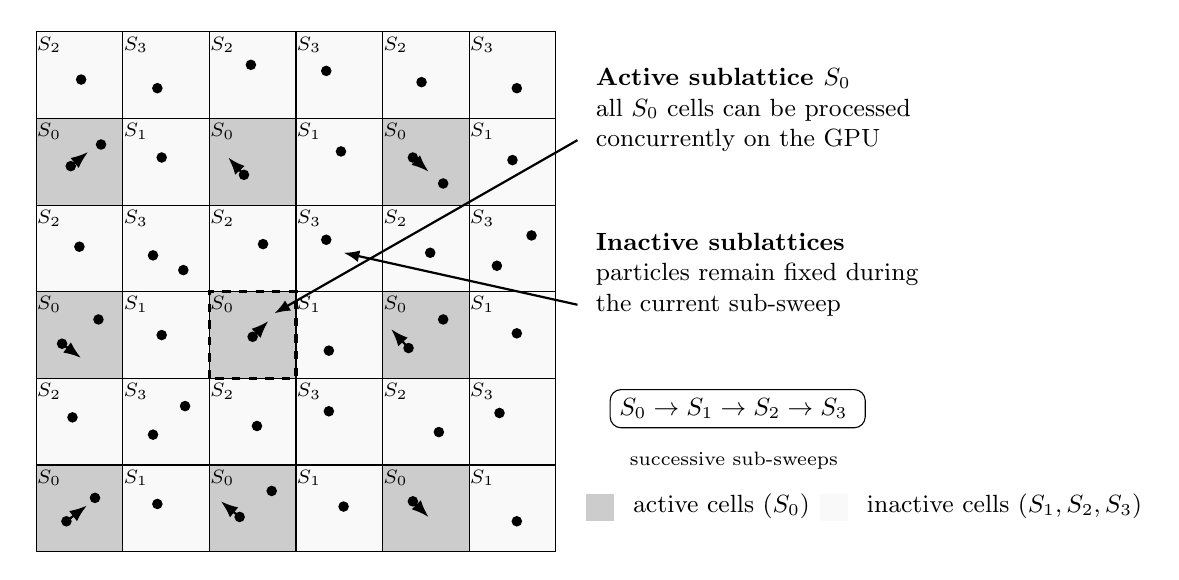
\begin{tikzpicture}[
    scale=1.00,
    particle/.style={circle, fill=black, inner sep=1.35pt},
    move/.style={-{Latex[length=2.2mm]}, thick},
    celllabel/.style={font=\scriptsize}
]

\def\a{1.10}

% -------------------------------------------------
% Four-sublattice checkerboard:
%
% S_2  S_3  S_2  S_3 ...
% S_0  S_1  S_0  S_1 ...
% S_2  S_3  S_2  S_3 ...
% S_0  S_1  S_0  S_1 ...
%
% alpha = mod(i,2) + 2*mod(j,2)
%
% Only sublattice S_0 is active in this sub-sweep.
% -------------------------------------------------

\foreach \i in {0,...,5}{
    \foreach \j in {0,...,5}{

        \pgfmathtruncatemacro{\px}{mod(\i,2)}
        \pgfmathtruncatemacro{\py}{mod(\j,2)}
        \pgfmathtruncatemacro{\sid}{\px+2*\py}

        % Active sublattice S_0
        \ifnum\sid=0
            \fill[gray!40]
              ({\i*\a},{\j*\a})
              rectangle
              ({(\i+1)*\a},{(\j+1)*\a});
        \else
            \fill[gray!5]
              ({\i*\a},{\j*\a})
              rectangle
              ({(\i+1)*\a},{(\j+1)*\a});
        \fi

        % Cell boundary
        \draw[thin]
          ({\i*\a},{\j*\a})
          rectangle
          ({(\i+1)*\a},{(\j+1)*\a});

        % Sublattice label
        \node[celllabel]
          at ({(\i+0.15)*\a},{(\j+0.85)*\a})
          {$S_{\sid}$};
    }
}

% -------------------------------------------------
% Particles
% -------------------------------------------------

% Row 0
\node[particle] at (0.35*\a,0.35*\a) {};
\node[particle] at (0.68*\a,0.62*\a) {};
\node[particle] at (1.40*\a,0.55*\a) {};
\node[particle] at (2.35*\a,0.40*\a) {};
\node[particle] at (2.72*\a,0.70*\a) {};
\node[particle] at (3.55*\a,0.52*\a) {};
\node[particle] at (4.35*\a,0.58*\a) {};
\node[particle] at (5.55*\a,0.35*\a) {};

% Row 1
\node[particle] at (0.42*\a,1.55*\a) {};
\node[particle] at (1.35*\a,1.35*\a) {};
\node[particle] at (1.72*\a,1.68*\a) {};
\node[particle] at (2.55*\a,1.45*\a) {};
\node[particle] at (3.38*\a,1.62*\a) {};
\node[particle] at (4.65*\a,1.38*\a) {};
\node[particle] at (5.35*\a,1.60*\a) {};

% Row 2
\node[particle] at (0.30*\a,2.40*\a) {};
\node[particle] at (0.72*\a,2.68*\a) {};
\node[particle] at (1.45*\a,2.50*\a) {};
\node[particle] at (2.50*\a,2.48*\a) {};
\node[particle] at (3.38*\a,2.32*\a) {};
\node[particle] at (4.30*\a,2.35*\a) {};
\node[particle] at (4.70*\a,2.68*\a) {};
\node[particle] at (5.55*\a,2.52*\a) {};

% Row 3
\node[particle] at (0.50*\a,3.52*\a) {};
\node[particle] at (1.35*\a,3.42*\a) {};
\node[particle] at (1.70*\a,3.25*\a) {};
\node[particle] at (2.62*\a,3.55*\a) {};
\node[particle] at (3.35*\a,3.60*\a) {};
\node[particle] at (4.55*\a,3.45*\a) {};
\node[particle] at (5.32*\a,3.30*\a) {};
\node[particle] at (5.72*\a,3.65*\a) {};

% Row 4
\node[particle] at (0.40*\a,4.45*\a) {};
\node[particle] at (0.75*\a,4.70*\a) {};
\node[particle] at (1.45*\a,4.55*\a) {};
\node[particle] at (2.40*\a,4.35*\a) {};
\node[particle] at (3.52*\a,4.62*\a) {};
\node[particle] at (4.35*\a,4.55*\a) {};
\node[particle] at (4.70*\a,4.25*\a) {};
\node[particle] at (5.50*\a,4.52*\a) {};

% Row 5
\node[particle] at (0.52*\a,5.45*\a) {};
\node[particle] at (1.40*\a,5.35*\a) {};
\node[particle] at (2.48*\a,5.62*\a) {};
\node[particle] at (3.35*\a,5.55*\a) {};
\node[particle] at (4.45*\a,5.42*\a) {};
\node[particle] at (5.55*\a,5.35*\a) {};

% -------------------------------------------------
% Trial moves: ONLY particles in active S_0 cells
% -------------------------------------------------

\draw[move]
  (0.35*\a,0.35*\a)
  -- ++(0.26,0.20);

\draw[move]
  (2.35*\a,0.40*\a)
  -- ++(-0.24,0.20);

\draw[move]
  (4.35*\a,0.58*\a)
  -- ++(0.20,-0.20);

\draw[move]
  (0.30*\a,2.40*\a)
  -- ++(0.24,-0.18);

\draw[move]
  (2.50*\a,2.48*\a)
  -- ++(0.20,0.20);

\draw[move]
  (4.30*\a,2.35*\a)
  -- ++(-0.22,0.24);

\draw[move]
  (0.40*\a,4.45*\a)
  -- ++(0.22,0.18);

\draw[move]
  (2.40*\a,4.35*\a)
  -- ++(-0.20,0.22);

\draw[move]
  (4.35*\a,4.55*\a)
  -- ++(0.20,-0.18);

% -------------------------------------------------
% Highlight one active S_0 cell
% -------------------------------------------------

\draw[very thick,dashed]
  (2*\a,2*\a)
  rectangle
  (3*\a,3*\a);

% -------------------------------------------------
% Explanation
% -------------------------------------------------

\node[
    align=left,
    font=\small,
    anchor=west
] at (6.35*\a,5.10*\a)
{
\textbf{Active sublattice $S_0$}\\
all $S_0$ cells can be processed\\
concurrently on the GPU
};

\draw[-{Latex[length=2mm]},thick]
  (6.25*\a,4.75*\a)
  -- (2.75*\a,2.75*\a);

\node[
    align=left,
    font=\small,
    anchor=west
] at (6.35*\a,3.20*\a)
{
\textbf{Inactive sublattices}\\
particles remain fixed during\\
the current sub-sweep
};

\draw[-{Latex[length=2mm]},thick]
  (6.25*\a,2.85*\a)
  -- (3.55*\a,3.45*\a);

% -------------------------------------------------
% Sublattice cycle
% -------------------------------------------------

\node[
    draw,
    rounded corners,
    align=center,
    font=\small
] at (8.1*\a,1.65*\a)
{
$S_0 \rightarrow S_1 \rightarrow S_2 \rightarrow S_3$
};

\node[
    align=center,
    font=\scriptsize
] at (8.1*\a,1.05*\a)
{
successive sub-sweeps
};

% -------------------------------------------------
% Legend
% -------------------------------------------------

\fill[gray!40]
  (6.35*\a,0.35*\a)
  rectangle ++(0.35,0.35);

\node[
    anchor=west,
    font=\small
] at (6.78*\a,0.52*\a)
{active cells ($S_0$)};

\fill[gray!5]
  (9.05*\a,0.35*\a)
  rectangle ++(0.35,0.35);

\node[
    anchor=west,
    font=\small
] at (9.48*\a,0.52*\a)
{inactive cells ($S_1,S_2,S_3$)};

\end{tikzpicture}

\caption{
Schematic representation of the four-sublattice checkerboard Monte
Carlo algorithm in two dimensions.
}
\label{fig:checkerboard_2d}
\end{figure*}



\section{Introduction}
\label{sec:intro}

Monte Carlo (MC) computer simulations represent a cornerstone of
computational physics, chemistry, and materials science
\cite{frenkel2001understanding,allen2017computer}. By stochastically
sampling configurations according to the Boltzmann distribution, MC
methods enable the calculation of equilibrium thermodynamic
observables, phase diagrams, free energy landscapes, and structural
correlation functions without requiring numerical integration of
equations of motion, bypassing kinetic bottlenecks that plague
Molecular Dynamics approaches in many instances. In the realm of soft
matter, complex fluids, and 
colloidal nanotechnology, MC simulations are indispensable for
investigating self-assembly, crystallization, gelation, and
liquid-liquid phase separation in isotropic fluids
\cite{carnahan1969equation}, patchy colloids
\cite{bianchi2006phase,sciortino2007patchy,noya2014phase,palaia2022patchy},
and dense multicomponent glass-forming liquids
\cite{ninarello2017models,berthier2017configurational}. 

Despite their theoretical generality, standard MC algorithms face two
narrow computational bottlenecks: 
\begin{enumerate}
    \item \textbf{Parallelization Constraints}: Unlike Molecular
      Dynamics (MD), where forces on all $N$ particles can be computed
      simultaneously in parallel
      \cite{anderson2008gpu,thompson2022lammps}, standard Metropolis
      MC algorithms evaluate sequential single-particle trial
      displacements, i.e., they are serial by construction. Modifying
      the position or orientation of particle 
      $i$ alters the local potential energy field, thereby
      invalidating concurrent moves of any neighboring particle $j$
      within the interaction cutoff distance $r_{\text{cut}}$. This
      sequential dependency has hindered so far the efficient
      exploitation of massively parallel graphics processing units
      (GPUs), in contrast with their widespread usage in Molecular
      Dynamics codes. 
    \item \textbf{Physical Kinetic Arrest}: In condensed systems,
      standard random particle translations and rotations resulting
      from either a Monte Carlo sweep or a Molecular Dynamics
      integration step frequently become trapped in local free-energy minima: 
    \begin{itemize}
        \item \emph{Steric Caging and Jamming}: In dense liquids and
          glass formers, particles are enclosed by rigid cages formed
          by nearest neighbors; translational displacements that yield
          reasonable acceptance rates ($30$--$50\%$) are constrained
          to fractions of an angstrom, leading to extremely slow diffusive
          relaxation \cite{ninarello2017models}, and the same applies
          to MD steps.  
        \item \emph{Entropic Bottlenecks in Dilute Associating
        Clusters}: In dilute patchy colloidal fluids ($V_{\text{box}}
          \gg V_{\text{clusters}}$), binding energies are strong
          ($\sim 10\,k_B T$). Gas-phase monomers spend huge
          numbers of Monte Carlo sweeps diffusing through empty space before
          randomly encountering an active cluster binding patch, while
          bonded particles rarely evaporate, which practically stops cluster size
          equilibration
          \cite{whitelam2007avoiding,rovigatti2018simulate}. 
        \item \emph{Compositional Freezing}: In multicomponent
          mixtures with non-additive diameters or asymmetric
          attractions, chemical species separation is arrested unless
          particles can interchange chemical identities without spatial
          diffusion
          \cite{ninarello2017models,berthier2017configurational}. 
    \end{itemize}
\end{enumerate}

To address parallelization, spatial domain decomposition
techniques—most notably the checkerboard algorithm—have
emerged as an effective paradigm for GPU acceleration
\cite{preis2009gpu,anderson2013checkerboard}. By partitioning the
simulation box into cells with linear dimensions larger than the
potential cutoff $r_{\text{cut}}$ and assigning cells to interleaved,
mutually non-interacting sublattices, thousands of trial moves can be
proposed and evaluated concurrently by independent CUDA thread blocks
without violating detailed balance. 

In this paper, we introduce \texttt{MCCB-gpu} (Monte Carlo
CheckerBoard on GPU), an open-source, high-throughput simulation
package written in CUDA Fortran and modern Fortran
2008. \texttt{MCCB-gpu} combines a 3D checkerboard GPU cellular engine
with: 
\begin{itemize}
    \item Full canonical ($NVT$) and isobaric-isothermal ($NpT$) ensemble sampling, with isotropic and anisotropic box volume trial moves.
    \item Broad potential support: athermal Hard Spheres (HS), continuous Lennard-Jones (LJ), arbitrary user-tabulated potentials (TABLE), angular patchy particles (Lennard-Jones-Gauss, LJG), and site-site patchy models for colloidal fluids (Palaia SSP model \cite{palaia2022patchy}) and biomolecular condensates (Sanchez-Burgos CSW/PHS model \cite{sanchezburgos2021size}) with quaternion rotational kinematics.
    \item Association Volume Bias Monte Carlo (AVBMC) \cite{chen2000avbmc,chen2001avbmc} guided by local geometric surface dipole asymmetry ($\eta_i \ge 0.5$) and coupled to a GPU implementation of G-DBSCAN (derived from the companion \texttt{trj\_analysis} package \cite{andrade2013gdbscan,trjanaly2026}).
    \item GPU-accelerated intra-cell and long-range cross-cell particle identity swaps ($A \leftrightarrow B$) for arbitrary multicomponent mixtures ($N_{\text{species}} \ge 2$).
    \item A high-efficiency, persistent in-memory Hybrid Monte Carlo (HMC) coupling layer with the LAMMPS molecular dynamics engine \cite{thompson2022lammps}, accelerating coordinate transfer by $287\times$ over disk I/O.
\end{itemize}

Several GPU-accelerated Monte Carlo simulation packages have been
developed in recent years. The GPU Optimized Monte Carlo (GOMC)
package \cite{Nejahi2019GOMC,Nejahi2021GOMC} provides a general
framework for molecular simulations and supports canonical ($NVT$),
isothermal--isobaric ($NpT$), grand-canonical ($\mu VT$), and Gibbs
ensembles, together with a broad range of all-atom, united-atom, and
coarse-grained force fields and advanced sampling schemes such as
configurational-bias and multi-particle Monte Carlo moves. In
contrast, \texttt{MCCB-gpu} is primarily targeted at simple and
multicomponent fluids, including additive and non-additive hard-sphere
mixtures, Lennard--Jones systems, arbitrary tabulated isotropic
potentials, and anisotropic patchy particles. As mentioned, a
distinctive feature of 
\texttt{MCCB-gpu} is that trial moves themselves are executed
concurrently on the GPU through a spatial checkerboard decomposition,
rather than limiting GPU acceleration to the evaluation of
interactions associated with sequentially proposed moves. This
strategy follows that of the massively parallel Metropolis Monte
Carlo approach introduced for hard particles and subsequently
implemented in the HPMC component of HOOMD-blue
\cite{Anderson2016HPMC}. \texttt{MCCB-gpu} extends this general approach
to energetic isotropic and orientation-dependent interactions and
provides GPU-parallel particle translations, rotations, and
identity-swap moves, as well as aggregation-volume-bias Monte Carlo
sampling for strongly associating systems. Thus, while GOMC
offers considerably broader ensemble coverage, molecular force-field
support, and a more mature simulation ecosystem, \texttt{MCCB-gpu}
occupies a complementary niche focused on massively concurrent
off-lattice Monte Carlo simulations of simple mixtures and anisotropic
patchy-particle systems. 



The remainder of this manuscript is organized as follows:
Section~\ref{sec:algorithms} details the mathematical formulations and
proofs of detailed balance for the checkerboard decomposition, AVBMC,
surface geometry identification, identity swaps, and
HMC. Section~\ref{sec:software} outlines the program architecture,
input namelists, and file formats. Section~\ref{sec:verification}
presents thermodynamic
consistency tests. Section~\ref{sec:benchmarks} discusses scaling and
computational performance. Section~\ref{sec:conclusions} concludes the
paper. 
\begin{table*}[tbp]
\centering
\small
\caption{\textbf{Control Parameters Namelist (\texttt{\&Control\_Params})}}
\label{tab:nml_control}
\begin{tabularx}{\textwidth}{l l c X}
\toprule
\textbf{Variable} & \textbf{Type} & \textbf{Default} & \textbf{Description / Physical Function} \\
\midrule
\texttt{istep\_ini} & Integer & 1 & Initial simulation sweep index (automatically updated in restarts). \\
\texttt{istep\_fin} & Integer & 1000 & Final simulation sweep index. \\
\texttt{Neq} & Integer & 0 & Number of equilibration sweeps (virial statistics excluded during equilibration). \\
\texttt{Nmove} & Integer & 125 & Trial moves attempted per active cell during each checkerboard sub-sweep. \\
\texttt{Nsave} & Integer & 100 & Frequency (in sweeps) for writing thermodynamic averages to \texttt{run-data.dat}. \\
\texttt{Ndump} & Integer & 1000 & Frequency (in sweeps) for appending frames to the trajectory file. \\
\texttt{Nrestart} & Integer & 5000 & Frequency (in sweeps) for writing restart checkpoints (\texttt{data.restart}). \\
\texttt{traj\_format} & Character & \texttt{'netcdf'} & Trajectory format: \texttt{'netcdf'} (binary NetCDF), \texttt{'plain'} (text XYZ/LAMMPS), or \texttt{'both'}. \\
\texttt{data\_file} & Character & \texttt{'data.atoms'} & Path to the initial atomic configuration file (LAMMPS data format). \\
\texttt{Npart\_types} & Integer & 1 & Number of distinct chemical species in the mixture ($N_{\text{species}}$). \\
\texttt{ncluster} & Integer & 0 & Frequency (in sweeps) for DBSCAN cluster analysis (0 = disabled). \\
\texttt{rcl} & Real & 1.8 & Radial neighbor connectivity threshold ($r_{\text{cl}}$) for cluster formation. \\
\texttt{minPts} & Integer & 3 & Minimum neighbor count for DBSCAN core node classification. \\
\texttt{asym\_threshold}& Real & 0.5 & Dipole asymmetry threshold ($\eta_{\text{thresh}}$) for cluster surface identification. \\
\texttt{cluster\_types}& Integer(10) & -1 & Species types included in cluster search (-1 = all species). \\
\texttt{avbmc} & Logical & \texttt{.false.} & Master flag to enable Association Volume Bias Monte Carlo moves. \\
\texttt{border\_criterion}& Character & \texttt{'asymmetry'}& Border identification method: \texttt{'asymmetry'} (geometric dipole) or \texttt{'energy'}. \\
\texttt{avbmc\_k\_trials}& Integer & 10 & Number of bulk Rosenbluth trial positions ($K$) per AVBMC attempt. \\
\texttt{avbmc\_max\_trials}& Integer & 50 & Maximum number of pair attempts per AVBMC invocation. \\
\texttt{lammps} & Logical & \texttt{.false.} & Master flag to enable in-memory Hybrid Monte Carlo moves via LAMMPS. \\
\bottomrule
\end{tabularx}
\end{table*}

\begin{table*}[tbp]
\centering
\small
\caption{\textbf{Monte Carlo Parameters Namelist (\texttt{\&MC\_Params})}}
\label{tab:nml_mc}
\begin{tabularx}{\textwidth}{l l c X}
\toprule
\textbf{Variable} & \textbf{Type} & \textbf{Default} & \textbf{Description / Physical Function} \\
\midrule
\texttt{temp0}, \texttt{temp1} & Real & 1.0, 1.0 & Initial and final temperatures ($T^*$ or Kelvin). Linear ramp if $\texttt{temp0} \neq \texttt{temp1}$. \\
\texttt{npt} & Logical & \texttt{.false.} & Master flag for isobaric-isothermal ($NpT$) ensemble sampling. \\
\texttt{pres} & Real & 0.0 & Target pressure ($P^*$ in reduced units or atmospheres in real units). \\
\texttt{Nvolf} & Integer & 1 & Frequency (in MC sweeps) of trial volume moves when \texttt{npt = .true.} \\
\texttt{hmax} & Real & 0.1 & Maximum trial displacement distance along Cartesian axes. \\
\texttt{omax} & Real & 0.1 & Maximum trial quaternion angular rotation parameter. \\
\texttt{vmax} & Real(3) & 0.01 & Maximum trial volume scaling factor along Cartesian axes. \\
\texttt{displ\_update} & Logical & \texttt{.false.} & Dynamically adjust \texttt{hmax} and \texttt{omax} to achieve $40\%$ acceptance. \\
\texttt{seed} & Integer & 123456 & Pseudo-random number generator seed. \\
\texttt{swap\_moves} & Logical & \texttt{.false.} & Enable GPU checkerboard particle identity swaps ($N_{\text{part\_types}} \ge 2$). \\
\texttt{Nswap} & Integer & 1 & Number of swap sub-passes executed per swap invocation. \\
\texttt{Nswapf} & Integer & 1 & Frequency (in MC sweeps) of identity swap moves. \\
\bottomrule
\end{tabularx}
\end{table*}



\begin{table*}[tbp]
\centering
\small
\caption{\textbf{Potential Parameters Namelist (\texttt{\&Potential\_Params})}}
\label{tab:nml_pot}
\begin{tabularx}{\textwidth}{l l c X}
\toprule
\textbf{Variable} & \textbf{Type} & \textbf{Default} & \textbf{Description / Physical Function} \\
\midrule
\texttt{model} & Character & \texttt{'LJ'} & Interaction potential: \texttt{'HS'}, \texttt{'LJ'}, \texttt{'TABLE'}, \texttt{'LJG'} (angular), \texttt{'SSP'} (Palaia site-site), or \texttt{'SB'} (Sanchez-Burgos site-site). \\
\texttt{table\_mc} & Logical & \texttt{.false.} & Use Catmull-Rom interpolated potential tables on the GPU. \\
\texttt{table\_file\_mc}& Character & \texttt{''} & Base prefix for MC potential table files (e.g., \texttt{'pot'} for \texttt{pot11.dat}). \\
\texttt{Bool\_tor} & Logical & \texttt{.false.} & Enable torsional angular patch modulation in LJG models. \\
\texttt{sigp\_factor} & Real & 0.1 & Patch width scaling factor in Palaia SSP models. \\
\texttt{Rcp\_factor} & Real & 0.3 & Patch radial cutoff scaling factor in Palaia SSP models. \\
\texttt{Rc\_factor} & Real & 2.0 & Core potential cutoff scaling factor in Palaia SSP models. \\
\texttt{patch\_radial\_factor}& Real & 0.5 & Distance from particle center to patch site ($r_p / \sigma$). \\
\texttt{eps\_R} & Real & 0.6667 & PHS core repulsive energy scale parameter ($\epsilon_R$) in SB model. \\
\texttt{eps\_CSW} & Real & 11.1111 & CSW patch attractive well depth ($\epsilon_{\text{CSW}} = 1/T^*$) in SB model. \\
\texttt{rw\_CSW} & Real & 0.12 & CSW patch attractive well width ($r_w / \sigma$) in SB model. \\
\texttt{alpha\_CSW} & Real & 0.005 & CSW patch well smoothing parameter ($\alpha / \sigma$) in SB model. \\
\texttt{rc\_CSW} & Real & 0.20 & CSW patch interaction radial cutoff ($r_c / \sigma$) in SB model. \\
\bottomrule
\end{tabularx}
\end{table*}

\begin{table*}[tbp]
\centering
\small
\caption{\textbf{LAMMPS Hybrid Monte Carlo Parameters Namelist (\texttt{\&Lammps\_Params})}}
\label{tab:nml_lammps}
\begin{tabularx}{\textwidth}{l l c X}
\toprule
\textbf{Variable} & \textbf{Type} & \textbf{Default} & \textbf{Description / Physical Function} \\
\midrule
\texttt{timestep} & Real & 0.0025 & MD integration timestep for HMC trajectory segments ($\Delta t$). \\
\texttt{Nmd} & Integer & 50 & Number of microcanonical MD steps executed per HMC trajectory segment. \\
\texttt{hmc\_freq} & Integer & 10 & Cadence (in MC sweeps) between successive HMC trajectory proposals. \\
\texttt{neigh\_skin} & Real & 0.3 & Neighbor list skin distance in LAMMPS distance units. \\
\texttt{thermo\_freq}& Integer & 0 & Frequency of internal LAMMPS thermodynamic logging (0 = disabled). \\
\texttt{use\_gpu} & Logical & \texttt{.true.} & Accelerate LAMMPS pair evaluation via the GPU package (\texttt{-pk gpu 1}). \\
\texttt{gpu\_id} & Integer & -1 & GPU device ID for LAMMPS (-1 = inherit \texttt{MCCB-gpu} active device). \\
\texttt{table\_lammps}& Logical & \texttt{.true.} & Force tabulated force representation in LAMMPS (\texttt{pair\_style table}). \\
\texttt{table\_file\_lammps}& Character & \texttt{''} & Filename prefix for LAMMPS tabulated potential files. \\
\bottomrule
\end{tabularx}
\end{table*}

\begin{figure*}[tbp]
\centering
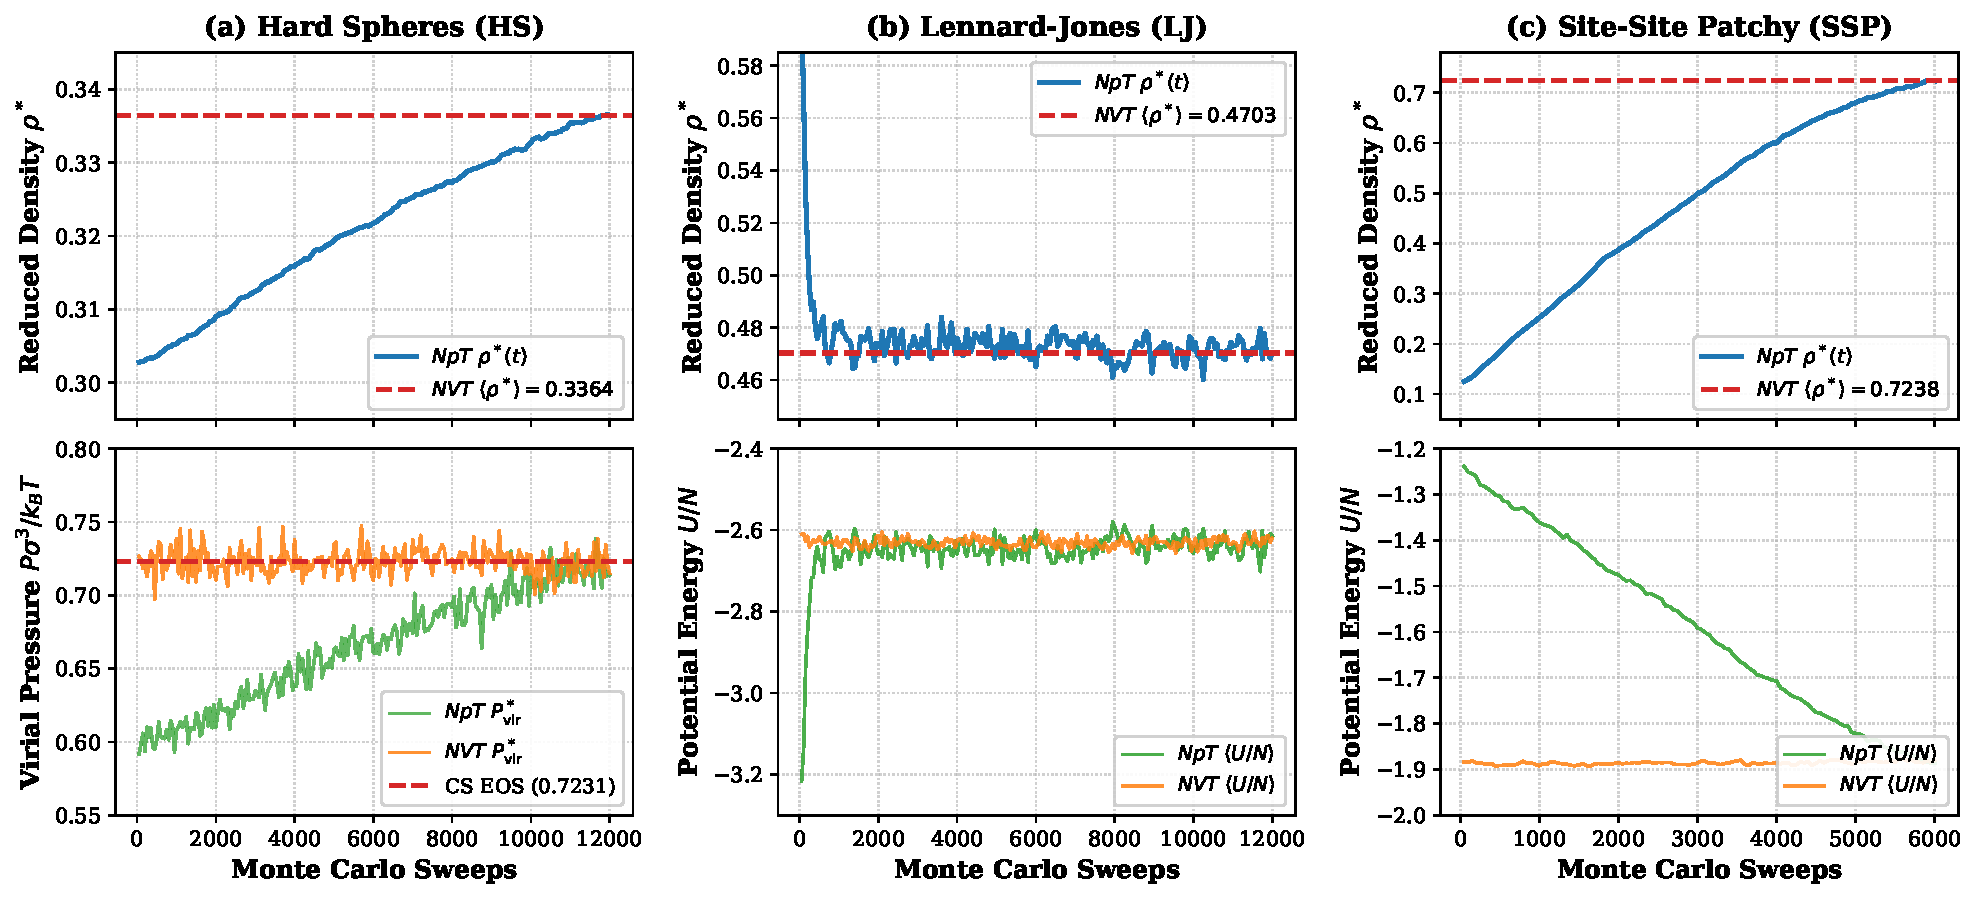
\includegraphics[width=\textwidth]{figures/consistency_all.pdf}
\caption{\textbf{Thermodynamic Consistency Benchmarks across $NpT$ and
    $NVT$ Ensembles for $N = 7{,}695$ Particles}: Time evolution of
  reduced density $\rho^*(t)$ (top row) and potential energy per
  particle $\langle U/N \rangle(t)$ or contact virial pressure
  $P^*(t)$ (bottom row) sharing the Monte Carlo sweep coordinate for:
  (a) Hard Spheres (HS) with analytical Carnahan-Starling
  equation-of-state verification, (b) Lennard-Jones (LJ), and (c)
  Site-Site Patchy (SSP) colloidal fluid, demonstrating exact
  statistical equivalence between ensembles.} 
\label{fig:consistency_all}
\end{figure*}



\section{Theoretical Formulation and Algorithms}
\label{sec:algorithms}

\subsection{3D Checkerboard Domain Decomposition}
\label{sec:algo_cb}

Consider a simulation domain of volume $V = L_x \times L_y \times L_z$
containing $N$ interacting bodies subject to periodic boundary
conditions (PBC). The interaction potential $U_{ij}$ vanishes beyond a
finite spherical cutoff distance $r_{\text{cut}}$, such that particles
separated by $r_{ij} \ge r_{\text{cut}}$ exert zero force and have
zero pairwise energy. 

To enable conflict-free concurrent evaluation on the GPU, \texttt{MCCB-gpu} discretizes the simulation volume into a regular Cartesian grid of $M_x \times M_y \times M_z = N_{\text{cells}}$ cells. The linear cell dimensions $L_{c,\alpha}$ satisfy:
\begin{equation}
    L_{c,\alpha} = \frac{L_\alpha}{M_\alpha} \ge r_{\text{cut}}, \quad \alpha \in \{x, y, z\}
    \label{eq:cell_condition}
\end{equation}
Cells are indexed by their discrete spatial coordinates $(c_x, c_y, c_z)$ with $c_\alpha \in \{0, \dots, M_\alpha - 1\}$. Each cell is assigned a color based on its 3D parity:
\begin{equation}
    \mathcal{C}(c_x, c_y, c_z) = (c_x \bmod 2) + 2(c_y \bmod 2) + 4(c_z \bmod 2)
    \label{eq:parity}
\end{equation}
with $\mathcal{C} \in \{0, \dots, 7\}$. This partitions the
$N_{\text{cells}}$ cells into 8 interleaved sublattices
$\mathcal{S}_0, \dots, \mathcal{S}_7$. Crucially, for any two distinct
cells $C_1, C_2 \in \mathcal{S}_\alpha$ belonging to the same sublattice,
their center-to-center separation along any Cartesian axis is at least
$2 L_{c,\alpha} \ge 2 r_{\text{cut}}$. Therefore, no particle in cell
$C_1$ can interact with any particle in cell $C_2$. A schematic
representation of the algorithm in 2D is shown in Figure~\ref{fig:checkerboard_2d}.
We see that the simulation domain is partitioned into spatial cells, each assigned 
to one of four sublattices $S_0$, $S_1$, $S_2$, or $S_3$ according to
the parity of its cell coordinates. Specifically, in 2D the sublattice
index is defined as
$\mathcal{C}(c_x, c_y) = (c_x \bmod 2) + 2(c_y \bmod 2)$, with a cell
$(c_x, c_y)$ belonging to $S_\alpha$ with $\alpha = \mathcal{C}(c_x, c_y)$.
During a given sub-sweep only one sublattice is active; here,
$S_0$ is shown in darker shading.
Particles located in different active cells can perform trial moves
simultaneously because active cells are spatially separated, while
particles belonging to the complementary sublattices remain fixed.
Successive sub-sweeps activate $S_1$, $S_2$, and $S_3$.
The two-dimensional construction is the direct analogue of the
$2\times2\times2$ eight-sublattice decomposition introduced above. 



A single Monte Carlo sweep consists of 8 sequential sub-sweeps (one
per sublattice $\mathcal{S}_k$). During sub-sweep $k$, a CUDA kernel
is launched where each thread block is assigned to an active cell $C
\in \mathcal{S}_k$. The thread block executes $N_{\text{move}}$ trial
moves within cell $C$. To evaluate the change in potential energy
$\Delta E$, the threads examine particles residing in cell $C$ and its
26 nearest-neighbor cells in the 3D grid. Because neighbor cells
belong to different sublattices $\mathcal{S}_{k'} \neq \mathcal{S}_k$,
their particle coordinates and occupancies are held strictly constant
during sub-sweep $k$. This guarantees zero read-write race conditions
across CUDA blocks, ensuring strict detailed balance without spinlocks
or thread synchronization.  

\subsection{Canonical (\texorpdfstring{$NVT$}{NVT}) and Isobaric-Isothermal (\texorpdfstring{$NpT$}{NpT}) Sampling}
\label{sec:algo_npt}

In the canonical ($NVT$) ensemble, trial moves consist of random
particle displacements $\mathbf{r}_i \to \mathbf{r}_i +
\delta\mathbf{r}$ with $\delta r_\alpha \in [-h_{\max},
  h_{\max}]$. For orientable bodies (patchy colloids, small
molecules), a rotational trial move is simultaneously proposed: 
\begin{equation}
    \mathbf{q}_i' = \frac{\mathbf{q}_i + \delta\mathbf{q}}{\|\mathbf{q}_i + \delta\mathbf{q}\|}
\end{equation}
where $\mathbf{q}_i \in \mathbb{S}^3$ is a unit quaternion and
$\delta\mathbf{q}$ is sampled uniformly over an angular range
controlled by parameter $o_{\max}$. The trial configuration is
accepted with Metropolis probability: 
\begin{equation}
    P_{\text{acc}} = \min\left(1, \, \exp(-\beta \Delta E)\right)
\end{equation}
where $\Delta E = E_{\text{new}} - E_{\text{old}}$ is computed
directly on the GPU streaming multiprocessors. 

In the isobaric-isothermal ($NpT$) ensemble, trial volume changes are
interleaved with particle displacement sweeps at cadence
$N_{\text{volf}}$. In isotropic mode, a volume change $\ln V \to \ln V
+ \delta v$ with $\delta v \in [-v_{\max}, v_{\max}]$ is proposed. The
box length scales as $L' = L (V'/V)^{1/3}$, and all particle
coordinates are rescaled affinely: 
\begin{equation}
    \mathbf{r}_i' = \left(\frac{V'}{V}\right)^{1/3} \mathbf{r}_i
\end{equation}
The volume change is accepted with probability:
\begin{multline}
    P_{\text{acc, vol}} = \min\Big(1, \, \exp\Big(-\beta \left[\Delta E_{\text{tot}} + P(V' - V)\right] \\
    + (N + 1)\ln\frac{V'}{V}\Big)\Big)
\end{multline}
where $\Delta E_{\text{tot}}$ is the total system energy difference,
recomputed via a parallel GPU reduction kernel. Following an accepted
volume move, the cell dimensions $L_{c,\alpha}$ are rescaled. If
$L_{c,\alpha}$ drops below $r_{\text{cut}}$, the grid multiplicity
$M_\alpha$ is automatically re-evaluated and the cellular neighbor
lists are refreshed. 

\paragraph{Virial Pressure for Hard Spheres}
For continuous potentials, pressure is evaluated via the standard
virial theorem (not implemented in the current program version). For
athermal Hard Spheres (HS), where impulsive forces 
preclude analytic derivatives, \texttt{MCCB-gpu} calculates the
instantaneous virial pressure via extrapolation of the radial
distribution function $g(r)$ to contact $r = \sigma^+$: 
\begin{equation}
    P_{\text{virial}}^{\text{HS}} = \rho k_B T \left[ 1 + \frac{2}{3}\pi \rho \sigma^3 g(\sigma^+) \right]
    \label{eq:hs_virial}
\end{equation}
During production, pairs are accumulated in fine radial histogram bins 
($dr = 0.002\sigma$), and $g(\sigma^+)$ is obtained via polynomial
extrapolation of a log-linear fitting all the way to contact values
\cite{Vrabecz2006}. This log-linear fitting improves accuracy for very
high packings for which the $g(r)$ slope near contact is huge. 

\subsection{Site-Site Patchy Interactions and Biomolecular Condensate Models}
\label{sec:algo_patchy_models}

For anisotropic bodies, \texttt{MCCB-gpu} supports explicit site-site architectures where a spherical core of diameter $\sigma$ is decorated with $M_p$ surface interaction sites (patches) positioned at radial distance $r_p = \xi \sigma$ (typically $\xi = 0.5$). Each patch coordinate $\mathbf{r}_{i,\alpha}$ is updated dynamically from the particle position $\mathbf{r}_i$ and orientation quaternion $\mathbf{q}_i$ via the rotation matrix $\mathbf{R}(\mathbf{q}_i)$:
\begin{equation}
    \mathbf{r}_{i,\alpha} = \mathbf{r}_i + \mathbf{R}(\mathbf{q}_i) \mathbf{p}_{i,\alpha}, \quad \alpha \in \{1, \dots, M_{p,i}\}
\end{equation}
where $\mathbf{p}_{i,\alpha}$ denotes the patch unit vector defined in the body-fixed reference frame. The total pairwise potential between particles $i$ and $j$ combines core-core repulsion and patch-patch attractive contributions:
\begin{equation}
    U_{ij} = U_{\text{core}}(r_{ij}) + \sum_{\alpha=1}^{M_{p,i}} \sum_{\beta=1}^{M_{p,j}} V_{\text{pot}}(\alpha, \beta) \, U_{\text{patch}}(\|\mathbf{r}_{i,\alpha} - \mathbf{r}_{j,\beta}\|)
    \label{eq:patchy_total}
\end{equation}
where $V_{\text{pot}}(\alpha, \beta) \in [0, 1]$ is a discrete compatibility matrix encoding chemical patch specificity.

In addition to the cosine-squared site-site model of Palaia and \v{S}ari\'{c} (\texttt{'SSP'}) \cite{palaia2022patchy}, \texttt{MCCB-gpu} implements the continuous square-well patchy model of Sanchez-Burgos \textit{et al.} (\texttt{'SB'}) \cite{sanchezburgos2021size}, developed to investigate liquid-liquid phase separation (LLPS) and size-conserved droplet condensation in scaffold-client protein mixtures. In this model, core-core steric repulsion is modeled by the Pseudo-Hard Sphere (PHS) potential:
\begin{equation}
    U_{\text{PHS}}(r) = \begin{cases}
        C \epsilon_R \left[ \left(\frac{\sigma}{r}\right)^{50} - \left(\frac{\sigma}{r}\right)^{49} \right] + \epsilon_R, & r < \frac{50}{49}\sigma \\
        0, & r \ge \frac{50}{49}\sigma
    \end{cases}
    \label{eq:u_phs}
\end{equation}
where $\epsilon_R = \frac{2}{3}$ is the repulsive energy scale and $C = 50 \left(\frac{50}{49}\right)^{49} \approx 136.0888$, which provides a continuous approximation to hard cores that vanishes smoothly with zero derivative at $r_c^{\text{PHS}} = \frac{50}{49}\sigma \approx 1.0204\sigma$. Patch-patch attraction is governed by the Continuous Square-Well (CSW) potential:
\begin{equation}
    U_{\text{CSW}}(d) = \begin{cases}
        -\frac{\epsilon_{\text{CSW}}}{2} \left[ 1 - \tanh\left(\frac{d - r_w}{\alpha}\right) \right], & d < r_c \\
        0, & d \ge r_c
    \end{cases}
    \label{eq:u_csw}
\end{equation}
where $d$ is the patch-patch Euclidean distance, $\epsilon_{\text{CSW}} = 1/T^*$ is the attractive well depth, $r_w = 0.12\sigma$ is the well radius, $\alpha = 0.005\sigma$ controls the well edge steepness, and $r_c = 0.20\sigma$ is the interaction cutoff. In a binary mixture, multivalent scaffold proteins feature 4 tetrahedral patches with self- and cross-affinity ($V_{\text{pot}} = 1.0$), while surfactant client proteins carry 3 coplanar patches with cross-affinity toward scaffolds ($V_{\text{pot}} = 1.0$) but zero client-client patch attraction ($V_{\text{pot}} = 0.0$), capping droplet growth and preserving finite condensate sizes.

\subsection{Association Volume Bias Monte Carlo (AVBMC)}
\label{sec:algo_avbmc}

In dilute colloidal and biomolecular fluids featuring strong directional attraction
(such as the site-site patchy models of Palaia and \v{S}ari\'{c}
\cite{palaia2022patchy} and Sanchez-Burgos \textit{et al.}
\cite{sanchezburgos2021size}), physical self-assembly leads to dense
clusters surrounded by an ultra-dilute monomer gas. Random translation
moves fail to equilibrate the cluster size distribution because the
probability of an isolated monomer encountering a free cluster binding
site 
scales as $V_{\text{bind}} / V_{\text{box}} \ll 10^{-3}$, while bound
particles experience deep potential wells ($U \sim -10\,k_B T$) that
prevent their vaporization in reasonable simulation times. 

To eliminate this entropic/energetic bottleneck, \texttt{MCCB-gpu}
incorporates Aggregation Volume Bias Monte Carlo
\cite{chen2000avbmc,chen2001avbmc}. AVBMC partitions configurational
space into a bonded binding region $V_{\text{bind}}$ around cluster
surfaces and the unbonded bulk volume $V_{\text{box}}$, proposing
direct macroscopic exchanges between these domains. 

\paragraph{Forward Association In-Move ($X \to Y$)}
Let $X$ denote a state with $N_{\text{free}}(X)$ gas-phase monomers and $N_{\text{brd}}(X)$ cluster border particles:
\begin{enumerate}
    \item A free monomer $i \in \mathcal{F}$ is selected uniformly:
      $P(i) = 1 / N_{\text{free}}(X)$. 
    \item A border particle $b \in \mathcal{B}$ is chosen uniformly:
      $P(b) = 1 / N_{\text{brd}}(X)$. 
    \item A target partner $t$ is selected uniformly from the
      $n_{\text{neigh}}(b)$ neighbors of $b$: $P(t) = 1 /
      n_{\text{neigh}}(b)$. 
    \item A trial position $\mathbf{r}'$ is sampled uniformly within
      the spherical binding volume $V_{\text{bind}} = \frac{4}{3}\pi
      r_{\text{bind}}^3$ centered at $\mathbf{r}_t$ ($r_{\text{bind}}
      = 1.5 r_{\text{cut}}$): $P(\mathbf{r}') = 1 / V_{\text{bind}}$. 
    \item To balance the bulk volume ratio, $K-1$ dummy trial
      positions $\{\mathbf{r}_m\}_{m=2}^K$ are generated uniformly in
      $V_{\text{box}}$, with trial 1 set to the current position
      $\mathbf{r}_i$. The bulk Rosenbluth sum is computed: 
    \begin{equation}
        W_{\text{bulk}} = 1 + \sum_{m=2}^K \exp\left(-\beta
        [E(\mathbf{r}_m) - E(\mathbf{r}_i)]\right) 
    \end{equation}
    \item The trial cluster Boltzmann weight is $w_{\text{cluster}} =
      \exp\left(-\beta [E(Y) - E(X)]\right)$. 
\end{enumerate}

\paragraph{Reverse Dissociation Out-Move ($Y \to X$)}
In state $Y$, particle $i$ resides at the cluster boundary, with $N_{\text{free}}(Y) = N_{\text{free}}(X) - 1$ and $N_{\text{brd}}(Y)$ border particles:
\begin{enumerate}
    \item Particle $i$ is selected from the border pool: $P(i) = 1 /
      N_{\text{brd}}(Y)$. 
    \item $K$ independent trial positions are generated uniformly in
      $V_{\text{box}}$. One trial corresponds to the original bulk
      location $\mathbf{r}_i$ (state $X$), with weight
      $w_{\text{rev}}(1) = \exp\left(-\beta [E(X) - E(Y)]\right) = 1 /
      w_{\text{cluster}}$. The reverse Rosenbluth sum is: 
    \begin{equation}
        W_{\text{bulk}}' = \sum_{m=1}^K w_{\text{rev}}(m) = \exp(\beta
        \Delta E) W_{\text{bulk}} 
    \end{equation}
    \item State $X$ is selected with probability $w_{\text{rev}}(1) /
      W_{\text{bulk}}'$. 
\end{enumerate}

\paragraph{Proof of Microscopic Reversibility}
Detailed balance requires $\pi(X) \alpha(X \to Y) P_{\text{acc}}(X \to Y) = \pi(Y) \alpha(Y \to X) P_{\text{acc}}(Y \to X)$, where $\pi(X) \propto e^{-\beta E(X)}$. The proposal probability densities are:
\begin{align}
    \alpha(X \to Y) &= \frac{1}{N_{\text{free}}(X)} \frac{1}{N_{\text{brd}}(X) n_{\text{neigh}}(b)} \frac{1}{V_{\text{bind}}} \left(\frac{1}{V_{\text{box}}}\right)^{K-1} \\
    \alpha(Y \to X) &= \frac{1}{N_{\text{brd}}(Y)} \left(\frac{1}{V_{\text{box}}}\right)^K \frac{e^{\beta \Delta E}}{W_{\text{bulk}}'}
\end{align}
The forward and reverse acceptance probabilities implemented in \texttt{MCCB-gpu} are:
\begin{align}
    P_{\text{acc}}(X \to Y) &= \min\left(1, \, \frac{N_{\text{brd}}(X) n_{\text{neigh}}(b) + 1}{N_{\text{free}}(X)} \frac{V_{\text{box}}}{V_{\text{bind}}} \frac{K w_{\text{cluster}}}{W_{\text{bulk}}}\right) \label{eq:avbmc_acc_fwd} \\
    P_{\text{acc}}(Y \to X) &= \min\left(1, \, \frac{N_{\text{free}}(Y) + 1}{N_{\text{brd}}(Y) n_{\text{neigh}}'} \frac{V_{\text{bind}}}{V_{\text{box}}} \frac{W_{\text{bulk}}'}{K}\right) \label{eq:avbmc_acc_rev}
\end{align}
Letting $\text{arg}_{\text{fwd}}$ and $\text{arg}_{\text{rev}}$ denote the arguments of the $\min(1, \cdot)$ functions, and noting that $N_{\text{free}}(Y) + 1 = N_{\text{free}}(X)$ and $W_{\text{bulk}}' = W_{\text{bulk}} / w_{\text{cluster}}$, their product satisfies:
\begin{equation}
    \text{arg}_{\text{fwd}} \cdot \text{arg}_{\text{rev}} \equiv 1
    \label{eq:avbmc_invariant}
\end{equation}
Because $\text{arg}_{\text{rev}} = 1 / \text{arg}_{\text{fwd}}$, it follows that:
\begin{equation}
    \frac{P_{\text{acc}}(X \to Y)}{P_{\text{acc}}(Y \to X)} = \frac{\min(1, \text{arg}_{\text{fwd}})}{\min(1, 1/\text{arg}_{\text{fwd}})} \equiv \text{arg}_{\text{fwd}}
\end{equation}
satisfying microscopic reversibility identically for any $K$, box volume $V_{\text{box}}$, and interaction model.

\subsection{Cluster Detection via G-DBSCAN and Surface Dipole Asymmetry}
\label{sec:algo_dbscan}

A core prerequisite for AVBMC is distinguishing cluster surface
particles from dense cluster interiors. Attempting to insert a monomer
into the deep interior of an assembled cluster invariably results in
steric overlap ($w_{\text{cluster}} = 0$). 

In \texttt{MCCB-gpu}, cluster identification is carried out on the GPU
using an implementation of \textsc{G-DBSCAN} (a GPU-accelerated
algorithm for density-based spatial clustering \cite{andrade2013gdbscan}),
directly adapted from the companion trajectory analysis package
\texttt{trj\_analysis} \cite{trjanaly2026}.  
Two particles $i$ and $j$ are defined as connected if their center-to-center distance (or patch-patch distance for SSP models) satisfies $r_{ij} \le r_{\text{cl}}$. The algorithm proceeds in two stages:
\begin{enumerate}
    \item \textbf{GPU Adjacency Graph Construction}: A CUDA kernel
      evaluates the neighborhood of each particle, populating compact
      adjacency arrays (\texttt{gneighbors}, \texttt{goffset},
      \texttt{gadjacency}) on device memory. Particles with neighbor
      counts $z_i \ge \text{minPts} - 1$ are classified as core
      candidates. 
    \item \textbf{Parallel BFS Expansion}: Connected components are
      identified via a GPU breadth-first search (\texttt{gbfs})
      kernel, assigning a unique \texttt{cluster\_id} to all particles
      in each cluster. 
\end{enumerate}

To isolate active surface sites, each particle $i$ in a cluster is evaluated using a local \textit{geometric dipole asymmetry parameter}, $\eta_i$:
\begin{equation}
    \eta_i = \frac{1}{z_i} \left\| \sum_{j \in \text{neigh}(i)} \hat{\mathbf{r}}_{ij} \right\|
    \label{eq:asym}
\end{equation}
where $\hat{\mathbf{r}}_{ij} = \mathbf{r}_{ij} / \|\mathbf{r}_{ij}\|$
is the unit bond vector pointing from particle $i$ to neighbor $j$,
and $z_i$ is the coordination number. 
\begin{itemize}
    \item \textbf{Core Particles}: Inside a cluster, neighbors
      surround particle $i$ nearly isotropically. The unit vectors
      cancel vectors in opposite hemispheres: $\sum_j
      \hat{\mathbf{r}}_{ij} \approx \mathbf{0}$, yielding $\eta_i
      \approx 0$. 
    \item \textbf{Surface/Border Particles}: At the cluster boundary,
      neighbors reside predominantly on one side. The sum of bond
      vectors does not cancel, producing a large net dipole vector
      with $\eta_i \ge \eta_{\text{thresh}} = 0.5$. 
\end{itemize}
Particles with $\eta_i \ge \eta_{\text{thresh}}$ are assigned to the
border pool $\mathcal{B}$, while unbonded particles ($z_i = 0$,
\texttt{cluster\_id} $= 0$) form the free pool
$\mathcal{F}$. Alternatively, an energy-based criterion ($u_i /
\langle u_{\text{bulk}} \rangle \le \text{ratio}$) is also available
via namelist control. 


\subsection{Multicomponent Particle Identity Swaps (\texorpdfstring{$A \leftrightarrow B$}{A <-> B})}
\label{sec:algo_swaps}

In dense multicomponent mixtures, such as non-additive hard sphere
(NAHS) fluids and binary glass formers, structural relaxation is
arrested by compositional jamming: particles cannot exchange positions
because intermediate steric barriers prevent physical
diffusion. Identity swap moves ($A \leftrightarrow B$) exchange the
species labels of two distinct particles while keeping their spatial
coordinates fixed, bypassing free-energy barriers along
compositional degrees of freedom. 

\texttt{MCCB-gpu} implements two complementary GPU checkerboard swap
kernels: 
\begin{enumerate}
    \item \textbf{Intra-Cell Swaps}: Within an active checkerboard
      cell $C$, two distinct particles $i, j \in C$ of different
      species ($S_i \neq S_j$) are chosen uniformly at random with
      probability: 
    \begin{equation}
        P_{\text{pair}}(i, j \mid C) = \frac{2}{n_C(n_C - 1)}
    \end{equation}
    where $n_C$ is the particle occupancy of cell $C$.
    \item \textbf{Cross-Cell Disjoint Swaps}: Two mutually
      non-adjacent active cells $C_1, C_2$ separated by $\ge
      r_{\text{cut}}$ are selected, and particles $i \in C_1, j \in
      C_2$ with $S_i \neq S_j$ are selected with probability $1 /
      (n_{C_1} n_{C_2})$. A symmetric random choice determines the
      swap direction. 
\end{enumerate}

\paragraph{Proof of Microscopic Reversibility}
Because particle coordinates are unchanged by identity swaps, the cell
occupancies $n_C$ are strictly invariant: 
\begin{equation}
    n_C(Y) = n_C(X) \implies \alpha_{\text{prop}}(Y \to X) \equiv \alpha_{\text{prop}}(X \to Y)
\end{equation}
The proposal ratio $\alpha(Y \to X)/\alpha(X \to Y)$ is identically
unity. For athermal hard spheres, the move is accepted if and only if
no hard-core overlaps are created. For continuous and patchy
potentials, the energy difference is: 
\begin{align}
    \Delta E &= \sum_{k \neq i, j} \left[ U(S_j, S_k, \mathbf{r}_{ik}) - U(S_i, S_k, \mathbf{r}_{ik}) \right] \nonumber \\
             &+ \sum_{k \neq i, j} \left[ U(S_i, S_k, \mathbf{r}_{jk}) - U(S_j, S_k, \mathbf{r}_{jk}) \right] + \Delta E_{ab}
\end{align}
where $\Delta E_{ab} = U(S_j, S_i, \mathbf{r}_{ij}) - U(S_i, S_j,
\mathbf{r}_{ij}) \equiv 0$ for symmetric pair interactions. The move
is accepted with standard Metropolis probability $\min(1, e^{-\beta
  \Delta E})$. 

\paragraph{Generalization to Multicomponent Mixtures ($N_{\text{species}} \ge 2$)}
In systems with $N_{\text{species}} > 2$, the two species labels $(A,
B)$ are chosen uniformly at random from all available pairs of
distinct species for each swap attempt. This preserves microscopic
reversibility across arbitrary ternary, quaternary, and polydisperse
mixtures. 

\subsection{Persistent In-Memory Hybrid Monte Carlo (HMC)}
\label{sec:algo_hmc}

To incorporate collective conformational rearrangements,
\texttt{MCCB-gpu} provides a Hybrid Monte Carlo (HMC) module
\cite{duane1987hybrid,mehlig1992hybrid} that periodically interleaves
canonical MC sweeps with microcanonical ($NVE$) Molecular Dynamics
(MD) trajectories generated by the LAMMPS engine
\cite{thompson2022lammps}. When implementing tabulated potentials,
those used for the Monte Carlo stage are stored in separate files from
those of the LAMMPS stage. This makes it possible to deal with long-range
potentials in the LAMMPS stage (that would otherwise inhibit the
checkerboard parallelization), while using the full power of the MC
algorithms for the short-range associative part of the
interactions. The current release does not implement Coulombic
interactions, but using an appropriate splitting of short-range vs
long-range components opens the path for an efficient implementation
in the future. 

Explicitly, here we start from an initial configuration
$\mathbf{q}_0$, with particle velocities $\mathbf{p}_0$ sampled
from 
the Maxwell-Boltzmann distribution at temperature $T$. A
microcanonical MD trajectory of $N_{\text{md}}$ timesteps is
integrated via the velocity Verlet algorithm. The final state
$(\mathbf{q}_\tau, \mathbf{p}_\tau)$ is accepted with generalized
Metropolis probability: 
\begin{equation}
    P_{\text{acc}}^{\text{HMC}} = \min\left(1, \, \exp\left(-\beta [\mathcal{H}(\mathbf{q}_\tau, \mathbf{p}_\tau) - \mathcal{H}(\mathbf{q}_0, \mathbf{p}_0)]\right)\right)
\end{equation}
where $\mathcal{H}(\mathbf{q}, \mathbf{p}) = U(\mathbf{q}) + \sum_i
\frac{\mathbf{p}_i^2}{2m_i}$ is the total classical Hamiltonian for
which the equations of motion have been integrated. 

\paragraph{Elimination of Disk and Task Forking Overheads}
Conventional implementations interface MC codes with LAMMPS by writing
ASCII data files (\texttt{lammps\_hmc.data}) to disk and invoking an
external binary or calling \texttt{clear} between trials. As
quantified in Section~\ref{sec:bench_hmc} and
Figure~\ref{fig:hmc_profile}, disk serialization and lexical parsing
consume $122.9$~ms per trial, while issuing \texttt{clear} incurs a
$351.5$~ms penalty to rebuild neighbor lists and reallocate GPU memory
buffers. 

\texttt{MCCB-gpu} resolves both bottlenecks by implementing a \textit{persistent in-memory architecture}:
\begin{enumerate}
    \item The LAMMPS instance, box topology, pair potentials, and GPU neighbor lists are initialized once during the first trial and maintained in host memory throughout the simulation.
    \item Coordinates are injected directly into LAMMPS via
      \texttt{lammps\_scatter\_atoms("x")} and extracted via
      \texttt{lammps\_gather\_atoms("x")}, completing in $0.43$~ms
      ($287\times$ faster than disk I/O). 
    \item For patchy particles, rigid bodies are projected onto
      central core atoms and satellite patch sites. Before each MD
      segment, periodic boundary image flags are zeroed (\texttt{set
        group all image 0 0 0}) and \texttt{fix rigid/nve molecule} is
      dynamically refreshed to prevent coordinate unwrap drift across
      successive HMC trials. 
\end{enumerate}

\section{Software Architecture and Program Description}
\label{sec:software}

\subsection{Modular Structure and Source Organization}
\label{sec:soft_arch}

\texttt{MCCB-gpu} is structured into modular compilation units
utilizing CUDA Fortran and Fortran 2008 with standard ISO C bindings: 
\begin{itemize}
    \item \texttt{src/Main.cuf}: Main simulation driver, command-line
      parsing, initialization, time evolution loop, periodic
      checkpointing, and clean shutdown. 
    \item \texttt{src/Subsweep\_Energy\_CUDA.cuf}: Core GPU
      computational engine containing the checkerboard sub-sweep
      kernels (\texttt{subsweep\_HS}, \texttt{subsweep\_LJ},
      \texttt{subsweep\_angular}, \texttt{subsweep\_sitesite}),
      identity swap kernels, and energy reduction routines. 
    \item \texttt{src/Cell.cuf} \& \texttt{src/cuda\_fortran.cuf}:
      Host and device data structures for 3D cellular grid indexing,
      particle coordinate packing, and GPU device memory allocations. 
    \item \texttt{src/mod\_clusters.cuf}: G-DBSCAN GPU neighbor
      search, parallel BFS traversal kernel (\texttt{gbfs}), and
      geometric dipole surface asymmetry calculation. 
    \item \texttt{src/mod\_avbmc.cuf}: AVBMC trial generator,
      Rosenbluth sum computation, and acceptance evaluation. 
    \item \texttt{src/lammps\_hmc\_wrapper.cuf}: C-API interface to
      \texttt{liblammps}, persistent memory management, coordinate
      scatter/gather, and rigid-body quaternion projection. 
    \item \texttt{src/potential\_functions.cuf}: Analytical pair interaction routines for continuous isotropic and site-site patchy models (\texttt{vphs}, \texttt{vcsw}, \texttt{vlj\_palaia}) equipped with dual host and device attributes.
    \item \texttt{src/Read\_input\_data\_nml.cuf}: Namelist parsing,
      input verification, and restart checkpoint writing
      (\texttt{input-restart.nml}). 
    \item \texttt{src/netcdf\_io.f90}: High-performance binary
      trajectory writer implementing the AMBER NetCDF convention
      (delivering $35\times$ file compression over text formats) also
      available in LAMMPS dumps. 
\end{itemize}

\subsection{Input Variables and Namelists}
\label{sec:soft_namelists}

Simulation parameters are provided via standard Fortran namelists in a
single input file (e.g.,
\texttt{datos.nml}). Tables~\ref{tab:nml_control}--\ref{tab:nml_lammps}
document all input variables, allowable values, and physical meanings. 

\begin{table*}[tbp]
\centering
\small
\caption{\textbf{Thermodynamic Consistency Validation across Interaction Models}}
\label{tab:thermo_consistency}
\begin{tabular*}{\textwidth}{@{\extracolsep{\fill}}l l c c c@{}}
\toprule
\textbf{Model} & \textbf{Observable} & \textbf{$NpT$ Ensemble} & \textbf{$NVT$ Ensemble} & \textbf{Discrepancy / Agreement} \\
\midrule
\textbf{Lennard-Jones} & Density $\langle \rho^* \rangle$ & $0.4723 \pm 0.0041$ & $0.4703$ & 0.43\% \\
($T^*=1.5, P^*=0.6$) & Energy $\langle U/N \rangle$ & $-2.640 \pm 0.023$ & $-2.631 \pm 0.011$ & \textbf{0.34\%} ($0.35\sigma$) \\
\midrule
\textbf{Hard Spheres} & Virial $P^*_{\text{NpT}}$ & $0.6767 \pm 0.0022$ & --- & \textbf{0.034\%} vs $P_{\text{CS}} = 0.67697$ \\
($T^*=1.0$) & Virial $P^*_{\text{NVT}}$ & --- & $0.7228 \pm 0.0006$ & \textbf{0.038\%} vs $P_{\text{CS}} = 0.72311$ \\
\midrule
\textbf{Site-Site Patchy} & Density $\langle \rho^* \rangle$ & $0.7158 \pm 0.0063$ & $0.7238$ & 1.11\% \\
($T^*=0.154, P^*=0.05$) & Energy $\langle U/N \rangle$ & $-1.873 \pm 0.010$ & $-1.885 \pm 0.003$ & \textbf{0.64\%} ($1.15\sigma$) \\
& Restart $U/N$ & $-1.88562$ & $-1.88560 \pm 0.0003$ & \textbf{0.001\%} (Exact Match) \\
\bottomrule
\end{tabular*}
\end{table*}


\subsection{Input and Output Files}
\label{sec:soft_files}

\paragraph{Input Files}
\begin{itemize}
    \item \texttt{datos.nml}: Primary input file containing namelists (\texttt{\&Control\_Params}, \texttt{\&MC\_Params}, \texttt{\&Potential\_Params}, \texttt{\&Lammps\_Params}) followed by pairwise interaction matrices ($\sigma_{ij}$, $\varepsilon_{ij}$, $r_{c,ij}$).
    \item \texttt{data.atoms}: Initial atomic configuration formatted according to the standard LAMMPS data specification, specifying box bounds, masses, and atomic coordinates (and quaternions for patchy models).
    \item \texttt{pot*.dat}: User-tabulated pairwise potential files (for \texttt{model = 'TABLE'}).
\end{itemize}

\paragraph{Output Files}
\begin{itemize}
    \item \texttt{run-data.dat}: Time series of thermodynamic observables: Step, Temperature, Density, Volume, $L_x$, $L_y$, $L_z$, and Potential Energy per atom.
    \item \texttt{trajectory.nc}: High-density binary NetCDF trajectory containing per-frame coordinates, quaternions, cell metrics, and metadata.
    \item \texttt{data.restart} \& \texttt{input-restart.nml}: Pair of exact checkpoint files capturing the full microstate and active simulation parameters, enabling seamless restarts without data loss.
    \item \texttt{clusevol\_mc.dat}: Time series of cluster statistics: Step, Cluster Count $N_{\text{clust}}$, Maximum Cluster Size $S_{\max}$, Clustered Particle Count, and Clustered Fraction (\%).
    \item \texttt{mclast\_conf.lammpstrj}: Final configuration formatted in LAMMPS trajectory format for visual analysis via VMD or OVITO.
\end{itemize}




\section{Verification and Algorithmic Validation}
\label{sec:verification}

Codes and reports for the verification tests listed below are included
with the software.

\subsection{Thermodynamic Consistency (\texorpdfstring{$NpT \leftrightarrow NVT$}{NpT <-> NVT})}
\label{sec:verif_consistency}

To verify the reliability of the code, in addition to checks with
literature data and other in-house codes, we perform a two-stage
workflow as follows:
\begin{enumerate}
    \item \textbf{Stage 1 ($NpT$)}: An isobaric-isothermal simulation
      is equilibrated at target pressure $P^*_{\text{target}}$ and
      temperature $T^*$, recording the mean volume $\langle V
      \rangle_{NpT}$ (density $\langle \rho^* \rangle_{NpT}$) and
      generating an exact checkpoint (\texttt{data.restart}). 
    \item \textbf{Stage 2 ($NVT$)}: A canonical simulation is executed
      from the restart configuration at fixed density $\rho^* =
      \langle \rho^* \rangle_{NpT}$. 
    \item \textbf{Validation}: Equivalence of internal potential
      energy $\langle U/N \rangle_{NVT} \approx \langle U/N
      \rangle_{NpT}$ is verified for continuous models, and virial
      pressure $\langle P_{\text{virial}} \rangle$ is cross-validated
      against the analytical Carnahan-Starling equation of state for
      Hard Spheres. 
\end{enumerate}


As summarized in Table~\ref{tab:thermo_consistency} and
Figure~\ref{fig:consistency_all}: 
\begin{itemize}
    \item For {\bf Hard Spheres}, the contact virial pressure reproduces the Carnahan-Starling equation of state \cite{carnahan1969equation}:
    \begin{equation}
        P_{\text{CS}}(\eta) = \rho k_B T \frac{1 + \eta + \eta^2 - \eta^3}{(1 - \eta)^3}, \quad \eta = \frac{\pi}{6}\rho\sigma^3
    \end{equation}
    within $\mathbf{0.034\%}$ in $NpT$ ($0.67674$ vs $0.67697$) and $\mathbf{0.038\%}$ in $NVT$ ($0.72284$ vs $0.72311$).
    \item For {\bf Lennard-Jones}, internal energies match with a discrepancy of only $0.34\%$ ($Z$-score of $0.35\sigma$).
    \item For {\bf Site-Site Patchy colloids}, internal energies match
      within $0.64\%$ ($Z = 1.15\sigma$), with exact configuration
      restart matching to within $0.001\%$. 
    \item For {\bf Biomolecular Condensates (Sanchez-Burgos Model)}, the implementation was cross-validated against an independent benchmark simulated in LAMMPS \cite{thompson2022lammps} for a binary 50:50 mixture of 2,000 scaffold and client proteins ($N = 2{,}000$, $\rho^* = 0.136$, $T^* = 0.09$). The initial total potential energy evaluated by \texttt{MCCB-gpu} ($-151.70959$) matches the LAMMPS benchmark ($-151.70991$) and the analytical Hamiltonian ($-151.71093$) with a relative discrepancy below $0.0002\%$, confirming exact consistency across CPU and GPU checkerboard implementations.
\end{itemize}

\subsection{Machine-Precision Numerical Verification of Detailed Balance}
\label{sec:verif_db}

To rigorously confirm that theoretical reversibility proofs translate
to error-free numerical implementations, independent automated test
harnesses were executed: 
\begin{enumerate}
    \item \textbf{AVBMC Invariant}: In an independent test harness
      evaluating 5,000 state transitions across Palaia patchy
      colloidal clusters, the flux reversibility invariant
      $|\text{arg}_{\text{fwd}} \cdot \text{arg}_{\text{rev}} - 1.0|$
      Eq.~\eqref{eq:avbmc_invariant} yielded a mean deviation of
      $\mathbf{3.17 \times 10^{-17}}$ and a maximum deviation of
      $\mathbf{4.44 \times 10^{-16}}$, matching IEEE 754 double
      precision machine epsilon ($\sim 2.22 \times 10^{-16}$). 
    \item \textbf{Identity Swaps}: Tested across $11{,}717$ intra-cell
      and cross-cell candidate transitions in dense non-additive hard
      sphere and continuous mixtures, the detailed balance residual
      $\delta_{\text{DB}} = |\pi(X)T(X\to Y) - \pi(Y)T(Y\to X)|$
      satisfied $\delta_{\text{DB}} < \mathbf{10^{-15}}$ with a
      $100.0\%$ pass rate. 
\end{enumerate}

\section{Performance Benchmarks and Discussion}
\label{sec:benchmarks}

\subsection{CPU vs. GPU Scaling: Normalizing Moves per Particle}
\label{sec:bench_cpu_gpu}

We benchmarked \texttt{MCCB-gpu} (v2.8.0) on an \textbf{NVIDIA RTX PRO
  4500 Blackwell GPU} (32 GB VRAM) against an optimized serial CPU
code \textbf{gpMC}~\cite{gpmc2026} (compiled with Intel Fortran
\texttt{ifx} 2025.2.0) on a 32-core \textbf{Intel Xeon Gold 6548Y+
  CPU} (2.20 GHz) for a binary Lennard-Jones mixture ($N_1{:}N_2 = 2{:}1$,
$T^* = 3.0$, $r_c = 2.5\sigma$) scaling from $N = 8{,}000$ to
$125{,}000$ particles for 100 MC sweeps. Larger sample sizes were
untreatable for the serial code.  

\paragraph{Normalization of Monte Carlo sweeps}
A critical methodological distinction between serial CPU code and
checkerboard GPU codes lies in the operational definition of a Monte
Carlo sweep: 
\begin{itemize}
    \item In \textbf{gpMC}, each sweep evaluates exactly 1 trial displacement per particle ($\mu_{\text{CPU}} = 1.0$).
    \item In \textbf{MCCB-gpu}, the checkerboard engine evaluates $N_{\text{move}} = 125$ trial moves per active cell across the 8 sublattices, attempting $N_{\text{trans}} = N_{\text{cells}} \times N_{\text{move}}$ moves per sweep. The number of moves attempted \emph{per particle per sweep} is:
    \begin{equation}
        \mu_{\text{GPU}} = \frac{N_{\text{cells}} \times N_{\text{move}}}{N}
    \end{equation}
    yielding $\mu_{\text{GPU}} = 3.375, 1.728, 1.953$, and $2.744$ moves/particle/sweep for $N = 8{,}000, 15{,}625, 32{,}768$, and $125{,}000$, respectively.
\end{itemize}
To provide an unbiased comparison of actual sampling throughput, we
report both the raw measured wallclock time $t_{\text{raw}}$ and the
normalized GPU runtime $t_{\text{norm}} = t_{\text{raw}} /
\mu_{\text{GPU}}$, along with the effective sampling speedup: 
\begin{equation}
    S_{\text{eff}} = \frac{t_{\text{CPU}}}{t_{\text{norm, GPU}}} = S_{\text{raw}} \times \mu_{\text{GPU}}
\end{equation}

\begin{figure}[tbp]
\centering
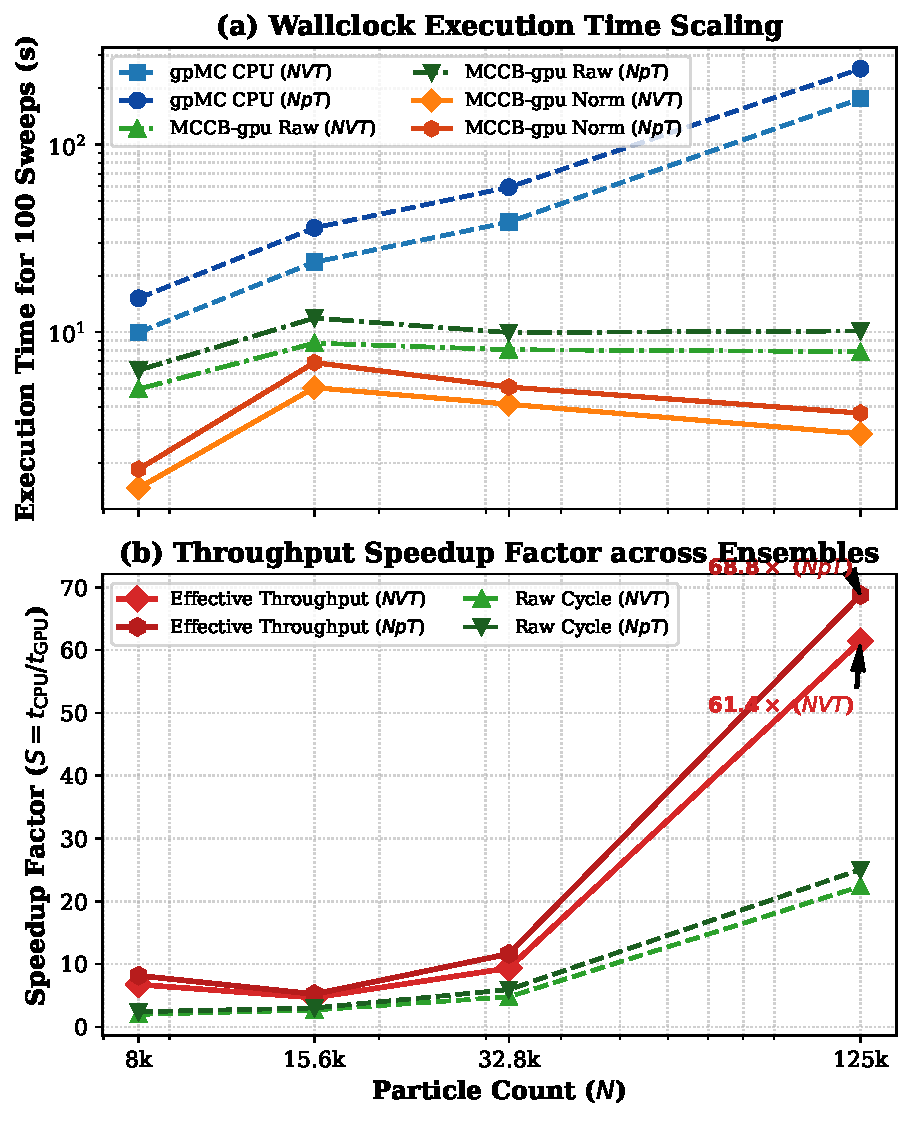
\includegraphics[width=\columnwidth]{figures/scaling_benchmark.pdf}
\caption{\textbf{gpMC (CPU) vs. MCCB-gpu (GPU) Performance Scaling across $NVT$ and $NpT$ Ensembles}: (a) Wallclock execution times for 100 sweeps on Intel Xeon Gold 6548Y+ vs. NVIDIA RTX PRO 4500. (b) Effective throughput speedup factor $S_{\text{eff}}$ accounting for moves per particle, reaching $61.4\times$ in $NVT$ and $68.8\times$ in $NpT$.}
\label{fig:scaling_bench}
\end{figure}

\begin{table*}[tbp]
\centering
\small
\caption{\textbf{Simulation Runtime (Seconds) and Speedup across CPU
    and GPU Architectures ($NVT$ and $NpT$ Ensembles) for a binary Lennard-Jones mixture ($N_1{:}N_2 = 2{:}1$, $T^* = 3.0$, $r_c = 2.5\sigma$)}}
\label{tab:gpmc_vs_mccbgpu}
\begin{tabular*}{\textwidth}{@{\extracolsep{\fill}}l c c c c c c c@{}}
\toprule
& \textbf{Moves/Part.} & \multicolumn{2}{c}{\textbf{gpMC CPU Time (s)}} & \multicolumn{2}{c}{\textbf{MCCB-gpu GPU Time (s)}} & \multicolumn{2}{c}{\textbf{Effective Speedup}} \\
\cmidrule{3-4} \cmidrule{5-6} \cmidrule{7-8}
\textbf{Particles ($N$)} & \textbf{($\mu_{\text{GPU}}$ / $\mu_{\text{CPU}}$)} & \textbf{$NVT$} & \textbf{$NpT$} & \textbf{$NVT$ (Norm)} & \textbf{$NpT$ (Norm)} & \textbf{$NVT$} & \textbf{$NpT$} \\
\midrule
\num{8000}   & 3.375 / 1.0 &   9.95 &  15.16 & 4.97 (1.47) &  6.26 (1.85) & \textbf{6.76$\times$} ($2.00\times$) & \textbf{8.17$\times$} ($2.42\times$) \\
\num{15625}  & 1.728 / 1.0 &  23.59 &  35.95 & 8.73 (5.05) & 11.88 (6.88) & \textbf{4.67$\times$} ($2.70\times$) & \textbf{5.23$\times$} ($3.03\times$) \\
\num{32768}  & 1.953 / 1.0 &  38.63 &  59.23 & 8.05 (4.12) &  9.94 (5.09) & \textbf{9.37$\times$} ($4.80\times$) & \textbf{11.64$\times$} ($5.96\times$) \\
\num{125000} & 2.744 / 1.0 & 175.91 & 254.09 & 7.86 (2.86) & 10.14 (3.70) & \textbf{61.41$\times$} ($22.39\times$) & \textbf{68.76$\times$} ($25.06\times$) \\
\bottomrule
\end{tabular*}
\end{table*}

As detailed in Table~\ref{tab:gpmc_vs_mccbgpu} and Figure~\ref{fig:scaling_bench}:
\begin{itemize}
    \item \textbf{Peak Speedup}: At $N = 125{,}000$, \texttt{MCCB-gpu} achieves raw speedups of $22.4\times$ ($NVT$) and $25.1\times$ ($NpT$). Accounting for moves per particle, the true sampling speedup reaches $\mathbf{61.4\times}$ in $NVT$ and $\mathbf{68.8\times}$ in $NpT$.
    \item \textbf{Anomalous GPU Saturation}: Between $N = 15{,}625$ and $N = 125{,}000$, GPU execution time remains essentially flat on the RTX PRO 4500 ($8.73 \to 7.86$~s in $NVT$, $11.88 \to 10.14$~s in $NpT$) despite an $8\times$ increase in particle count! This plateau demonstrates peak CUDA warp occupancy and block memory coalescing on modern GPU architectures.
\end{itemize}

\subsection{Large-Scale Scaling: LAMMPS vs. MCCB-gpu}
\label{sec:bench_large}

Table~\ref{tab:lammps_vs_mccb} evaluates scaling up to nearly four
million particles ($N \approx 4 \times 10^6$) comparing
\texttt{MCCB-gpu} against GPU-accelerated LAMMPS on NVIDIA RTX 2000
and RTX 4500 hardware for a binary Lennard-Jones mixture ($N_1{:}N_2 = 2{:}1$,
$T^* = 3.0$, $r_c = 2.5\sigma$). \texttt{MCCB-gpu} maintains
linear $\mathcal{O}(N)$ scaling, executing 100 sweeps for $3.94 \times
10^6$ particles in just $25.6$~s on the RTX 4500. 

\begin{table}[htbp]
\centering
\caption{\textbf{Large-Scale Simulation Runtimes (Seconds for 100
    Steps) for a binary Lennard-Jones mixture ($N_1{:}N_2 = 2{:}1$, $T^* = 3.0$, $r_c = 2.5\sigma$)}}
\label{tab:lammps_vs_mccb}
\resizebox{\columnwidth}{!}{%
\begin{tabular}{l c c c c}
\toprule
& \multicolumn{2}{c}{\textbf{LAMMPS Time (s)}} & \multicolumn{2}{c}{\textbf{MCCB-gpu Time (s)}} \\
\cmidrule(lr){2-3} \cmidrule(lr){4-5}
\textbf{Particles ($N$)} & \textbf{RTX 2000} & \textbf{RTX 4500} & \textbf{RTX 2000} & \textbf{RTX 4500} \\
\midrule
\num{492450}  &  7.0 &  5.0 &  18.0 &  3.8 \\
\num{1969920} & 22.0 & 18.0 &  66.0 & 13.2 \\
\num{3939840} & 44.0 & 34.0 & 123.0 & 25.6 \\
\bottomrule
\end{tabular}%
}
\end{table}

\begin{figure*}[!t]
\centering
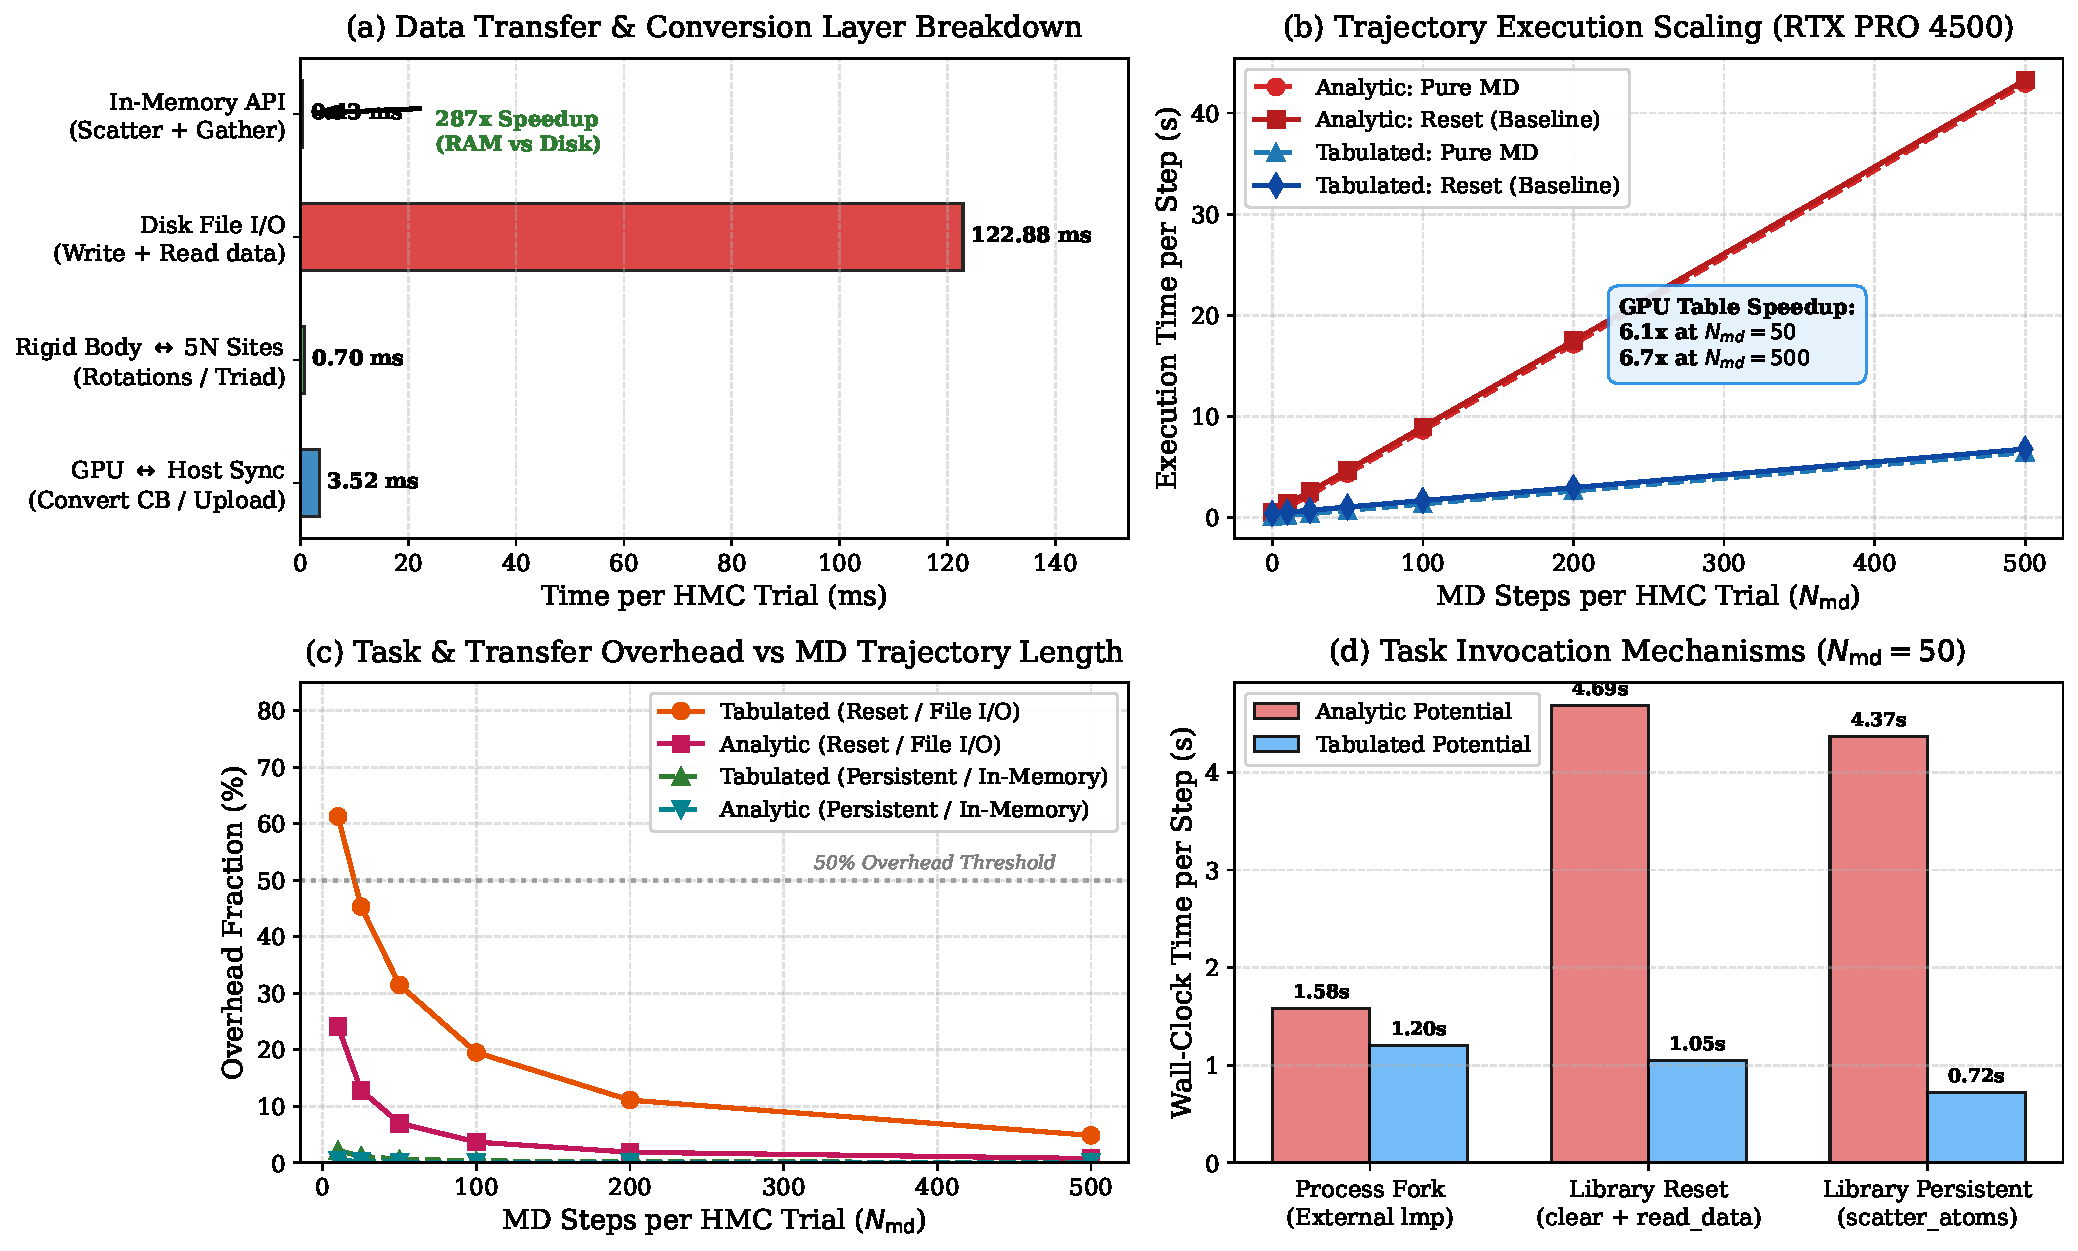
\includegraphics[width=0.96\textwidth]{figures/hmc_overhead_benchmark_comparison.pdf}
\caption{\textbf{Profiling of In-Memory HMC Coupling with LAMMPS on
    NVIDIA RTX PRO 4500}: (a) Latency breakdown showing the
  $287\times$ speedup of direct in-memory C-API coordinate transfer
  ($0.43$~ms) over disk ASCII file I/O ($122.9$~ms). (b) MD trajectory
  propagation scaling with $N_{\text{md}}$, highlighting a
  $6.1\times$--$6.7\times$ throughput advantage for GPU-accelerated
  tabular potentials over analytic overlays. (c) Coupling overhead
  fraction versus $N_{\text{md}}$. (d) Comparison of task invocation
  paradigms for $N_{\text{md}} = 50$ steps.} 
\label{fig:hmc_profile}
\end{figure*}

\subsection{In-Memory Hybrid Monte Carlo Overhead Breakdown}
\label{sec:bench_hmc}

Profiling the HMC coupling layer for $N = 7{,}695$ tetrahedral patchy colloids ($38{,}475$ explicit interaction sites) reveals:
\begin{itemize}
    \item \textbf{Data Transfer Acceleration}: Writing and parsing
      ASCII data files to disk consumes $122.88$~ms per trial
      ($96.7\%$ of baseline transfer time). Direct in-memory pointer
      transfers via \texttt{scatter\_atoms} and \texttt{gather\_atoms}
      require only $0.43$~ms—a $\mathbf{287\times}$ acceleration. 
    \item \textbf{Persistent State Optimization}: Eliminating
      in-process \texttt{clear} calls saves $351.5$~ms of neighbor
      list and memory allocation overhead per trial, delivering a
      $1.66\times$ overall speedup. 
    \item \textbf{Crossover Length}: For GPU-accelerated tabulated
      potentials, physical MD integration begins to dominate over
      coupling overhead at $N_{\text{md}}^* \approx 20$ timesteps. 
\end{itemize}

\subsection{Sampling Acceleration: AVBMC and Identity Swaps}
\label{sec:bench_advanced_moves}

\begin{figure}[tbp]
\centering
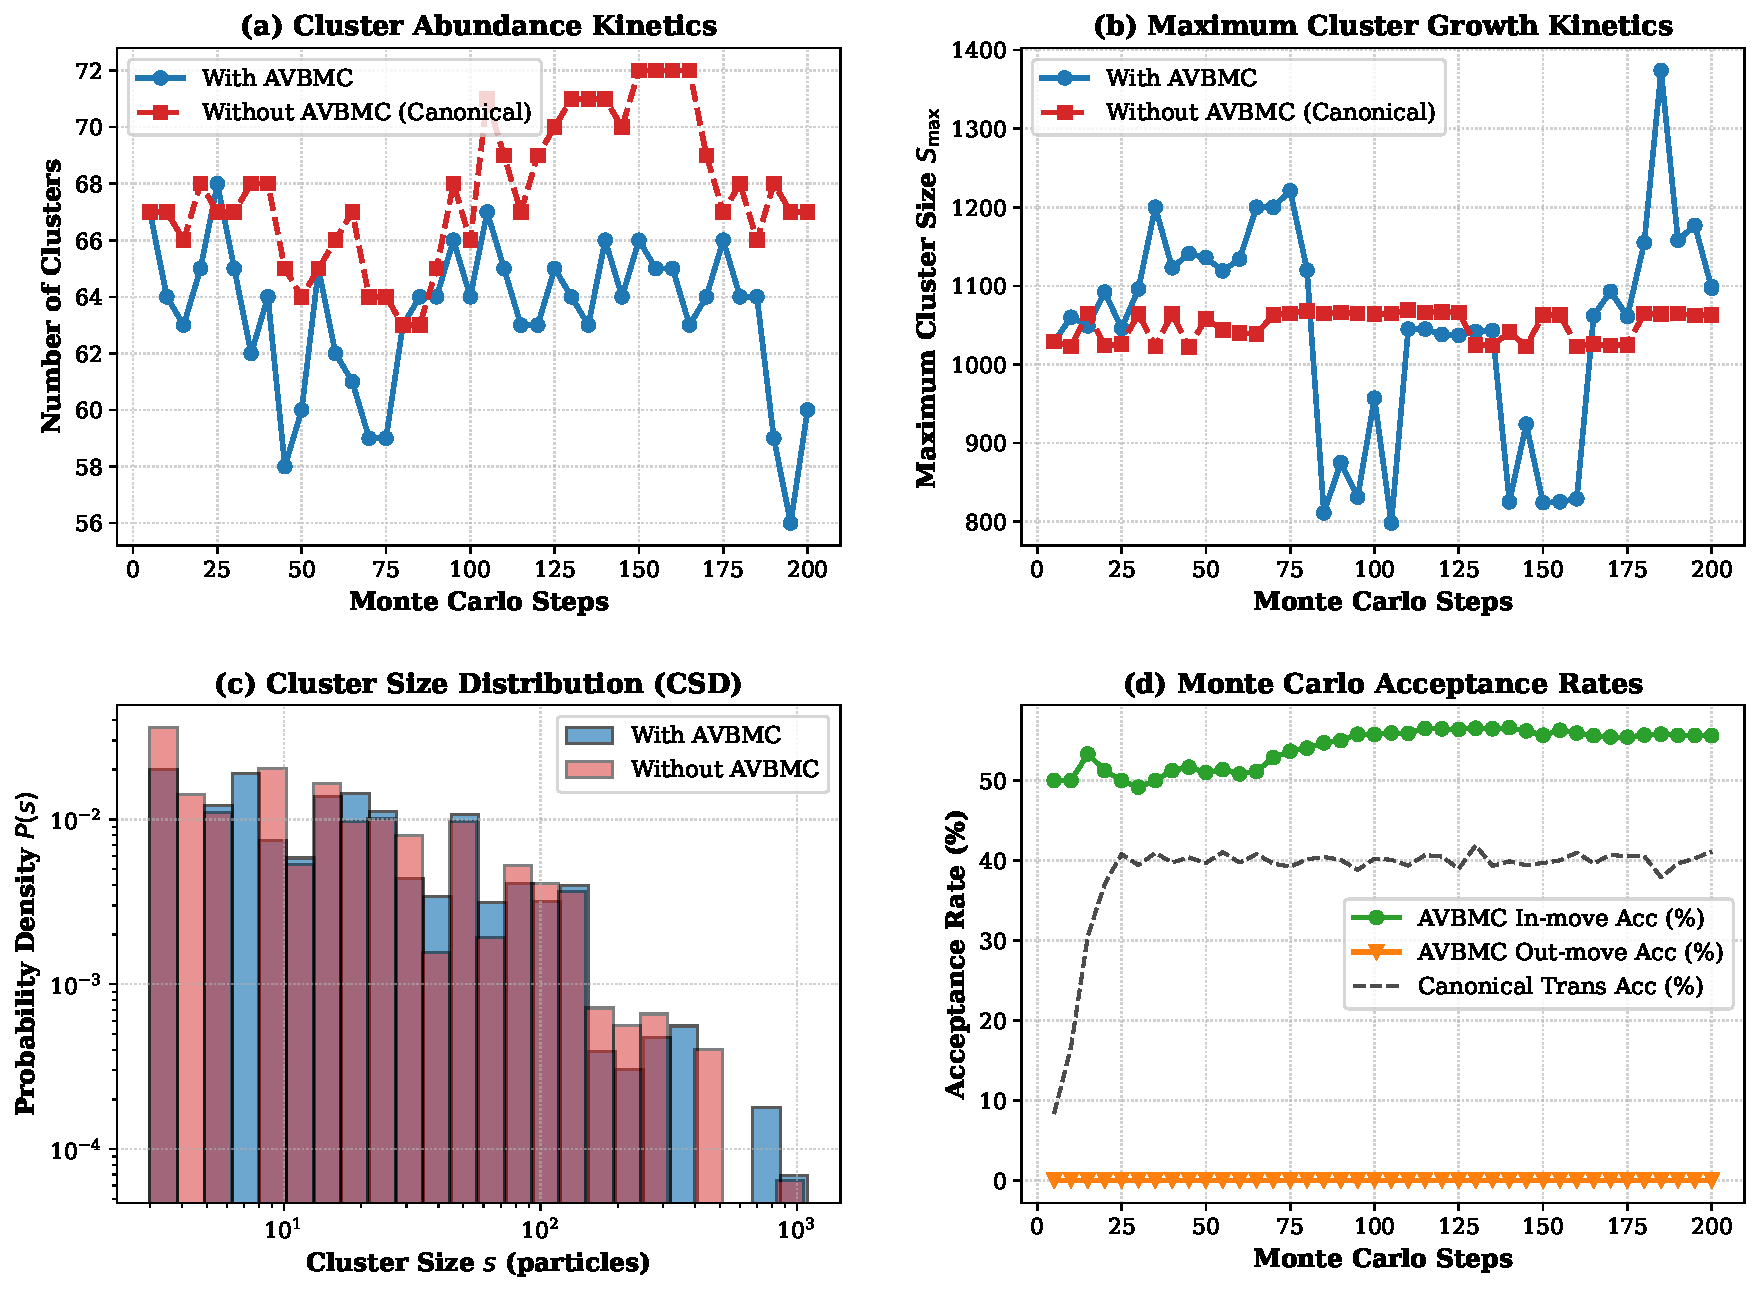
\includegraphics[width=\columnwidth]{figures/avbmc_benchmark_comparison.pdf}
\caption{\textbf{Comparative Benchmark of Patchy Colloidal Cluster
    Sampling With vs. Without AVBMC}: (a) Maximum cluster size
  evolution $S_{\max}(t)$ demonstrating accelerated aggregation
  kinetics and overcoming kinetic traps. (b) Monte Carlo acceptance
  rates for association ($P_{\text{AV,in}}$), dissociation
  ($P_{\text{AV,out}}$), and standard canonical displacement
  ($P_{\text{trans}}$), sharing the Monte Carlo simulation steps
  coordinate.} 
\label{fig:avbmc_bench}
\end{figure}

\begin{figure}[tbp]
\centering
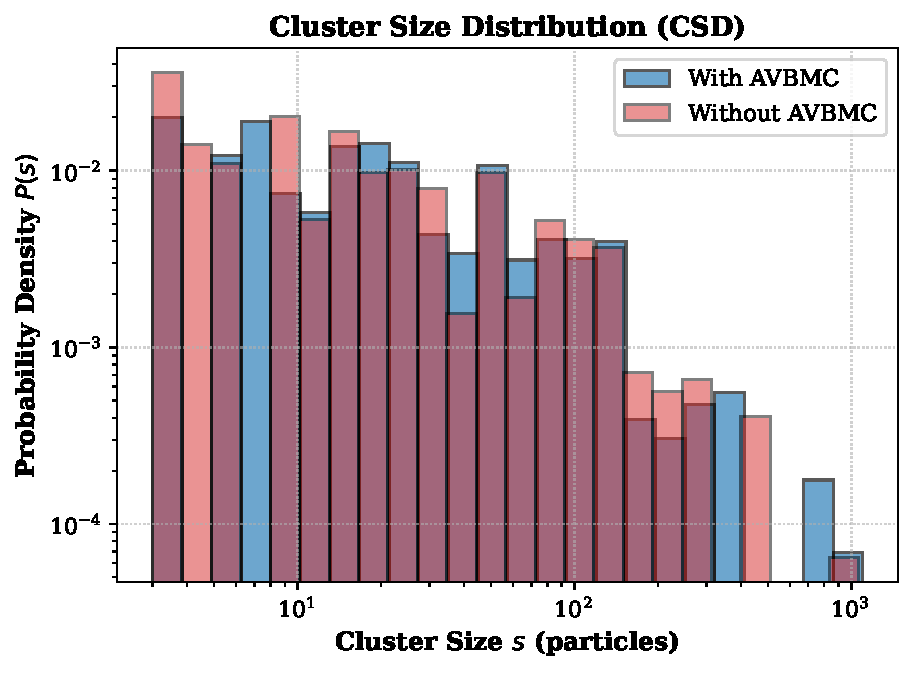
\includegraphics[width=\columnwidth]{figures/avbmc_csd_distribution.pdf}
\caption{\textbf{Final Cluster Size Distribution (CSD) for Patchy
    Colloids With vs. Without AVBMC}: Normalized probability $P(s)$
  versus cluster size $s$ after 200 sweeps, highlighting that AVBMC
  significantly accelerates aggregation into large macromolecular
  clusters ($s > 500$) compared to kinetically arrested canonical
  sampling.} 
\label{fig:avbmc_csd}
\end{figure}

\paragraph{AVBMC on Patchy Colloidal Clusters}
As shown in Figures~\ref{fig:avbmc_bench} and~\ref{fig:avbmc_csd}, in
a dilute binary patchy colloidal fluid ($N = 7{,}695$, $\rho =
0.001218$, $T^* = 0.154$), standard canonical MC undergoes kinetic
arrest: the maximum cluster size stagnates at $S_{\max} \approx 1068$,
and the clustered fraction declines as monomers evaporate into the
void.  

With AVBMC enabled, the association acceptance rate reaches
$P_{\text{AV,in}} = \mathbf{55.6\%}$ (Figure~\ref{fig:avbmc_bench}b),
transferring over 440 monomers directly to active cluster surface
sites over 200 sweeps and driving cluster growth to $S_{\max} = 1374$
(Figure~\ref{fig:avbmc_bench}a). As evidenced by the cluster size
distribution in Figure~\ref{fig:avbmc_csd}, AVBMC actively populates
the tail of large assemblies ($s > 500$). Remarkably, the
computational overhead of performing G-DBSCAN clustering and 800 AVBMC
trial moves every 5 sweeps is under $\mathbf{2.8\%}$ ($473.7$~ms/sweep
vs $460.5$~ms/sweep). 

\paragraph{Identity Swaps in Jammed Non-Additive Mixtures}
In a dense non-additive hard sphere mixture ($N = 2{,}916$, $P^* =
70.24$), canonical simulations exhibit completely frozen compositional
sampling: the species autocorrelation function defined as 
\begin{equation}
    C_s(\Delta t) = \frac{\langle (s_i(t_0 + \Delta t) - \bar{s})(s_i(t_0) - \bar{s}) \rangle}{\text{Var}(s)}
\end{equation}
where $s_i(t) \in \{+1, -1\}$ denotes the species identity of particle
$i$ at time $t$, and the average $\langle \dots \rangle$ is taken over
all $N$ particles and time origins $t_0$, remains $C_s(\Delta t) \equiv
1$ and zero particles exchange chemical identities. With GPU 
identity swaps enabled, $41.4\%$ of particles exchange species labels,
rapidly decaying $C_s(\Delta t)$ to $0.45$. This dramatic ergodicity
restoration introduces only $+1.02$~ms/sweep ($+18.6\%$) in GPU
latency across more than 71 million attempted swap moves. 

\section{Conclusions}
\label{sec:conclusions}

We have introduced \texttt{MCCB-gpu}, an open-source, massively
parallel GPU Monte Carlo simulation code for soft-matter and molecular
modeling. By combining a 3D checkerboard domain decomposition with
three targeted sampling algorithms—AVBMC guided by geometric dipole
surface asymmetry, multicomponent particle identity swaps, and
persistent in-memory Hybrid Monte Carlo/LAMMPS—\texttt{MCCB-gpu}
bridges the gap between massive GPU parallel efficiency and advanced
free-energy sampling.  

The tests confirm the thermodynamic consistency between
$NpT$ and $NVT$ ensembles. Accuracy for hard spheres has been tested
against analytical EoS ($< 0.04\%$). Additive and non-additive hard
sphere mixtures were tested against the results of the DynamO
hard-core event-driven simulation engine~\cite{bannerman2011dynamo}. 
Benchmarking against an optimized serial CPU
Monte Carlo code demonstrates algorithmic sampling throughput speedups
up to $\mathbf{68.8\times}$ on modern NVIDIA GPUs. Testing against
LAMMPS results for site-site patchy models and simple mixtures, both
using analytical and tabulated potentials, confirms the reliability of
the results. The source code,
complete documentation, automated test suites, and tutorials are
freely available under the GPLv3 license at
\url{https://github.com/adpozuelo/MC_Checkerboard}. 

\section{Declaration of generative AI and AI-assisted technologies in
  the manuscript preparation process} 

During the preparation of this work the authors used Gemini 3.8 in
order to generate input parameter and output file tables, performance
checks and figures, the latter under the strict guidance of the
authors. After using this tool, the authors 
reviewed and edited the content as needed and take full
responsibility for the content of the published article. During
revision, the authors also used OpenAI Codex to compare the repository
changes with the manuscript and assist with updating the text,
equations and parameter tables. During the implementation of the
software, the authors have used OpenAI Codex to assist in the design
of the algorithm for hard sphere simulations, Gemini 3.8 to refactor
and document the code, and to implement the AVBMC and identity swap
algorithms. These code implementations were double-checked for
thermodynamic internal consistency, and against Molecular Dynamics
results from LAMMPS for continuous potentials and DynamO for hard
sphere mixtures~\cite{bannerman2011dynamo}.


\section*{Declaration of Competing Interest}
The authors declare that they have no known competing financial
interests or personal relationships that could have appeared to
influence the work reported in this paper. 

\section*{Acknowledgements}
\enlargethispage{2\baselineskip}
This work was supported by the Spanish Ministry of Science, Innovation
and Universities (MICIU/AEI/10.13039/501100011033) and by ``ERDF A way
of making Europe'' through Grant PID2023-151751NB-I00. Computational
resources were provided by the high-performance computing clusters at
the Instituto de Qu{\'{i}}mica F{\'{i}}sica Blas Cabrera (IQF-CSIC)
and the Galicia Supercomputing Center (CESGA).  

\bibliographystyle{elsarticle-num}
\bibliography{references}

\vspace{1.5em}
\hrule
\vspace{1em}


\end{document}
